\documentclass[10pt]{article}


\usepackage[czech]{babel}
\usepackage{a4wide}
\usepackage[utf8]{inputenc}
\usepackage[T1]{fontenc}
\usepackage{fancyhdr}
\usepackage{amssymb}
\usepackage{amsmath}
\usepackage{mathtools}
\usepackage{mleftright}
\usepackage{hyperref}
\usepackage{titlesec}
%This has to be the last
\usepackage{subfiles}

\usepackage{geometry}
\geometry{
    a4paper,
    total={170mm,257mm},
    right=20mm,
    left=20mm,
    top=30mm,
    bottom=20mm,
}

\DeclareMathOperator{\rank}{rank}
\DeclareMathOperator{\Span}{span}

\titleformat{\section} {\normalfont\fontsize{16}{15}\bfseries}{\thesection}{1em}{}
\titleformat{\subsection} {\normalfont\fontsize{14}{15}\bfseries}{\thesubsection}{1em}{}
\titleformat{\subsubsection} {\normalfont\fontsize{12}{15}\bfseries}{\thesubsubsection}{1em}{}

\pagestyle{fancy}
\fancyhf{}
%\lhead{Viktor Soukup, Lukáš Salak}
\rhead{Matematická analýza II}
\fancyfoot{}
\fancyfoot[R]{\thepage}

\begin{document}

\begin{titlepage}
    \begin{center}
        \vspace*{1cm}
            
        \Huge
        \textbf{Matematická analýza II}
            
        \vspace{0.5cm}
        \LARGE
        Stručné výpisky
            
        \vspace{1.5cm}
            
        \textbf{Viktor Soukup, Lukáš Salak}
        
        \vfill
        \flushright
        \normalsize
        Bez revize, první verze \\
        Leden 2021
        
    \end{center}
\end{titlepage}

\tableofcontents
\clearpage

%%%%%%%%%%%%%%%%%%%%%%%%%%%%%%%%%%%%%%%%%%%%%%%%%%%%%%%%%%%%%%%%%%%%%%%%%%%%%%%%%%%%%%%%%%%%%%%%%%%%%%%%%
\section{Metrické prostory}
%%%%%%%%%%%%%%%%%%%%%%%%%%%%%%%%%%%%%%%%%%%%%%%%%%%%%%%%%%%%%%%%%%%%%%%%%%%%%%%%%%%%%%%%%%%%%%%%%%%%%%%%%
\subsection{Definice metrického prostoru}
\large
\hspace{1.2mm}
Metrický prostor : $(X,d), d: X \times X \rightarrow \mathbb{R}$, kde platí:

\begin{itemize}
\item{$d(x,y \geq 0, d(x,y) \iff x = y$ }
\item{$d(x,y) = d(y,x)$}
\item{$d(x,z) \leq d(x,y) + d(y,z)$ (trojúhelníková nerovnost)}
\end{itemize}
\noindent


\hspace{1.2mm}
Příklady: 
\[(\mathbb{R}, |x-y|),\]
\[(\mathbb{C},|x-y|)\]
\hspace{1.2mm}
Pozor: trojúhelníková nerovnost v $(\mathbb{C}, |x-y|)$ není tak triviální jako v $\mathbb{R}$.
\noindent
%%%%%%%%%%%%%%%%%%%%%%%%%%%%%%%%%%%%%%%%%%%%%%%%%%%%%%%%%%%%%%%%%%%%%%%%%%%%%%%%%%%%%%%%%%%%%%%%%%%%%%%%%
\subsection{Euklidovský prostor $\mathbb{E}_n$}
\hspace{1.2mm}
Definujeme jako $(\mathbb{R}^n,d)$, kde $d$:
\[d((x_1,...,x_n),(y_1,...,y_n)) = \sqrt{\sum_i(x_i-y_i)^2}\]

Pro nás zvlášť důležitý, známy v podobě vektorového prostoru $\textbf{V}_n$ se skalárním součinem $\textbf{u}v$ a normou
$||\textbf{u}|| = \sqrt{\textbf{uu}}$ a vzdáleností $||\textbf{u}-\textbf{v}||$
\noindent

%%%%%%%%%%%%%%%%%%%%%%%%%%%%%%%%%%%%%%%%%%%%%%%%%%%%%%%%%%%%%%%%%%%%%%%%%%%%%%%%%%%%%%%%%%%%%%%%%%%%%%%%%
\subsection{Diskrétní prostor}
\hspace{1.2mm}
Definujeme jako $(X,d)$, kde $d(x,y) = 1$ pro $x \neq y$
\noindent

%%%%%%%%%%%%%%%%%%%%%%%%%%%%%%%%%%%%%%%%%%%%%%%%%%%%%%%%%%%%%%%%%%%%%%%%%%%%%%%%%%%%%%%%%%%%%%%%%%%%%%%%%
\subsection{Podprostor}
\hspace{1.2mm}
\noindent
Buď $(X, d)$ metrický prostor. Pak $(Y, d')$ je podprostor, kde $Y \subseteq X$ a $d'(x,y) = d(x,y)$.

%%%%%%%%%%%%%%%%%%%%%%%%%%%%%%%%%%%%%%%%%%%%%%%%%%%%%%%%%%%%%%%%%%%%%%%%%%%%%%%%%%%%%%%%%%%%%%%%%%%%%%%%%
\subsection{Spojité zobrazení}
\hspace{1.2mm}
\noindent

$f: (X,d) \to (Y, d')$ je spojité zobrazení, pokud
\[ \forall x \in X, \forall \epsilon > 0 \exists \delta > 0:
d(x,y) < \delta \Rightarrow d'(f(x), f(x)) < \epsilon \]

\subsection{Triviality}
\subsubsection{Identické zobrazení}

\[ (X,d) \to (X,d) \]

\subsubsection{Vložení podprostoru}

\[ j = (x \mapsto x): (Y,d') \to (X,d) \]

\subsubsection{Složení spojitých zobrazení je spojité}

Pokud jsou $f: (X,d) \to (Y, d')$ a $g: (Y,d') \to (Z, d'')$ spojité, pak i
\[ g \circ f: (X,d) \to (Z,d'') \] je spojité.

%%%%%%%%%%%%%%%%%%%%%%%%%%%%%%%%%%%%%%%%%%%%%%%%%%%%%%%%%%%%%%%%%%%%%%%%%%%%%%%%%%%%%%%%%%%%%%%%%%%%%%%%%
\subsection{Věta o konvergenci}
\hspace{1.2mm}
Zobrazení $f: (X_1,d_1) \rightarrow (X_2,d_2)$ je spojité právě když pro každou konvergentní $(x_n)_n v (X_1,d_1)$ 
posloupnost $(f(x_n))_n$ konverguje v $(X_2,d_2)$ a platí $\lim_n f(x_n) = f(\lim_n x_n)$.

Důkaz:
Buď $f$ spojitá a nechť $\lim_nx_n = x$. Pro $\epsilon > 0$ svolme ze spojitosti $\delta > 0$
tak aby $d_2(f(y),f(x)) <\epsilon$ pro $d_1(x,y) < \delta$.
Podle definice konvergence posloupnosti existuje $n_0$ takové, že pro $n\geq n_0$ je $d_1(x_n,x) < \delta$. Tedy je-li $n \leq n_0$
máme $d_2(f(x_n),f(x)) < \epsilon$ a potom $\lim_n f(x_n) = f(\lim_n x_n)$.
\noindent


%%%%%%%%%%%%%%%%%%%%%%%%%%%%%%%%%%%%%%%%%%%%%%%%%%%%%%%%%%%%%%%%%%%%%%%%%%%%%%%%%%%%%%%%%%%%%%%%%%%%%%%%%
\subsection{Okolí}
\hspace{1.2mm}
\noindent
$\Omega (x,\epsilon) = \{ y | d(x,y) < \epsilon \}$

\vspace{5mm}

\textbf{Užití:}
$"\textrm{U je okolí } x" \equiv \exists \epsilon > 0, \Omega (x,\epsilon) \subseteq U $

%%%%%%%%%%%%%%%%%%%%%%%%%%%%%%%%%%%%%%%%%%%%%%%%%%%%%%%%%%%%%%%%%%%%%%%%%%%%%%%%%%%%%%%%%%%%%%%%%%%%%%%%%
\subsection{Otevřená a uzavřená množina}
\hspace{1.2mm}
\noindent
$U \subseteq (X,d)$ je \textbf{otevřená}, pokud je okolím \textit{každého} svého bodu.

\vspace{5mm}

\hspace{1.2mm}
\noindent $V \subseteq (X,d)$ je \textbf{uzavřená}, pokud $\forall (x_n)_n \subseteq A$ je konvergentní
v $X$ je $\lim_n x_n$ v $A$.

%%%%%%%%%%%%%%%%%%%%%%%%%%%%%%%%%%%%%%%%%%%%%%%%%%%%%%%%%%%%%%%%%%%%%%%%%%%%%%%%%%%%%%%%%%%%%%%%%%%%%%%%%
\subsection{Uzávěr}
\hspace{1.2mm}
\noindent
\textbf{Uzávěr} $A$ je $\overline{A} = \{ x | d(x,A) = 0 \}$

%%%%%%%%%%%%%%%%%%%%%%%%%%%%%%%%%%%%%%%%%%%%%%%%%%%%%%%%%%%%%%%%%%%%%%%%%%%%%%%%%%%%%%%%%%%%%%%%%%%%%%%%%
\subsection{Vlastnosti zobrazení mezi metrickými prostory}
\hspace{1.2mm}
\noindent
Buďte $(X_1, d_1)$ a $(X_2, d_2)$ metrické prostory a buď zobrazení $f: X_1 \to X_2$. Následující
jsou potom ekvivalentní:
\begin{enumerate}
    \item $f$ je spojité.
    \item $\forall x \in X_1$ a $\forall$ okolí $V$ bodu $f(x)$ existuje okolí $U$ bodu $x$ takové, že
        $f[U] \subseteq V$.
    \item $\forall$ otevřenou $U$ v $X_2$ je vzor $f^{-1}[U]$ otevřený v $X_1$.
    \item $\forall$ uzavřenou $A$ v $X_2$ je vzor $f^{-1}[U]$ uzavřený v $X_1$.
    \item $\forall A \subseteq X_1$ je $f[\overline{A}] \subseteq \overline{f[A]}$
\end{enumerate}


%%%%%%%%%%%%%%%%%%%%%%%%%%%%%%%%%%%%%%%%%%%%%%%%%%%%%%%%%%%%%%%%%%%%%%%%%%%%%%%%%%%%%%%%%%%%%%%%%%%%%%%%%
\subsection{Silně ekvivalentní metriky}
\hspace{1.2mm}
\noindent
Buďte $d_1, d_2$ metriky. $d_1$ a $d_2$ na téže jsou silně ekvivalentní, pokud
\[\exists \alpha , \beta > 0: \alpha d_1(x,y) \leq d_2(x,y) \leq \beta d_1(x,y)\]

%%%%%%%%%%%%%%%%%%%%%%%%%%%%%%%%%%%%%%%%%%%%%%%%%%%%%%%%%%%%%%%%%%%%%%%%%%%%%%%%%%%%%%%%%%%%%%%%%%%%%%%%%
\subsection{Vzory a obrazy}
\hspace{1.2mm}
$f: X \rightarrow Y, A \subseteq X, B \subseteq Y$
\noindent
%%%%%%%%%%%%%%%%%%%%%%%%%%%%%%%%%%%%%%%%%%%%%%%%%%%%%%%%%%%%%%%%%%%%%%%%%%%%%%%%%%%%%%%%%%%%%%%%%%%%%%%%%
\subsubsection{Obraz}
\hspace{1.2mm}
\underline{Obraz} podmnožiny $A\subseteq X$ v $Y$:
\[f[A] = \{f(x) | x \in A\}\]
\noindent

%%%%%%%%%%%%%%%%%%%%%%%%%%%%%%%%%%%%%%%%%%%%%%%%%%%%%%%%%%%%%%%%%%%%%%%%%%%%%%%%%%%%%%%%%%%%%%%%%%%%%%%%%
\subsubsection{Vzor}
\hspace{1.2mm}
\underline{Vzor} podmnožiny $B\subseteq Y$ v $X$:
\[f^{-1}[B] = \{x | f(x) \in B\}\]

\[X \underset{f^{-1}[-]}{\stackrel{f[-]}{\rightleftarrows}} Y\]

Platí:
\[f[A] \subseteq B \equiv A \subseteq f^{-1}[B],\]
\[f[f^{-1}[B]] \subseteq B  ...  f^{-1}[f[A]] \supseteq A\]


\textbf{Pozor:} $f^{-1}$ má dvá významy:
\begin{itemize}
    \item inverze $f^{-1}:Y \rightarrow X$, nemusí existovat
    \item část v symbolu $f^{-1}[-]$, má smysl vždy
 
\end{itemize}
\noindent

%%%%%%%%%%%%%%%%%%%%%%%%%%%%%%%%%%%%%%%%%%%%%%%%%%%%%%%%%%%%%%%%%%%%%%%%%%%%%%%%%%%%%%%%%%%%%%%%%%%%%%%%%
\subsection{Reálná funkce o $n$ proměnných}
\hspace{1.2mm}
\[f: D \rightarrow \mathbb{R}, D \subseteq \mathbb{E}_n\]

Podobně jako ve funkcích jedné proměnné se nemůžeme omezit na případy, kdy definiční obor je celý prostor $\mathbb{E}_n$. V 
Případě funkcí jedné proměnné byly definiční obory obvykle intervaly nebo jednoduchá sjednocení intervalů. Tady budou definiční
obory $D$ složitější, často (ale né vždy) otevřené množiny v $\mathbb{E}_n$.

O $D$ se často mluví jako o oblasti na níž je funkce definovaná. To není termín (ve specifických kontextech slovo "oblast" termín 
je, tady ne).
\noindent

%%%%%%%%%%%%%%%%%%%%%%%%%%%%%%%%%%%%%%%%%%%%%%%%%%%%%%%%%%%%%%%%%%%%%%%%%%%%%%%%%%%%%%%%%%%%%%%%%%%%%%%%%
\subsection{Součiny}
\hspace{1.2mm}
Pro $(X_1,d_i), i = 1,...,n$ definujeme na kartézskem součinu $\prod^n_{i=1}X_i$ metriku
\[d((x_1,...,x_n),(y_1,...,y_n)) = \max_i d_i(x_i,y_i)\].

Získaný
\[\left(\prod^n_{i=1}X_i,d_i\right) = \prod^n_{i=1}(X_i,d_i)\]

se nazývá součin prostorů $(X_i, d_i)$. Píše se též 
\[(X_1,d_1) \times \cdot \cdot \cdot \times (X_n,d_n).\]
\noindent

%%%%%%%%%%%%%%%%%%%%%%%%%%%%%%%%%%%%%%%%%%%%%%%%%%%%%%%%%%%%%%%%%%%%%%%%%%%%%%%%%%%%%%%%%%%%%%%%%%%%%%%%%
\subsection{Věta o spojitých zobrazeních}
\begin{enumerate}
\item Projekce $p_j = ((x_i)_i \mapsto x_j) : \prod^n_{i=1}(X_i,d_i) \rightarrow (X_j,d_j)$ jsou spojitá zobrazení.

\item Buďte $f_j:(Y,d') \rightarrow (X_j,d_j)$ libovolná spojitá zobrazení. Potom jednoznačně určené zobrazení 
$f:(Y,d') \rightarrow \prod^n_{i=1}(X_i,d_i)$ splňujíci $p_j \circ f = f_j$, totiž zobrazení definované předpisem
$f(y) = (f_1(y),...,f_n(y))$, je spojité.
\end{enumerate}

Jak to vypadá:
\begin{center}
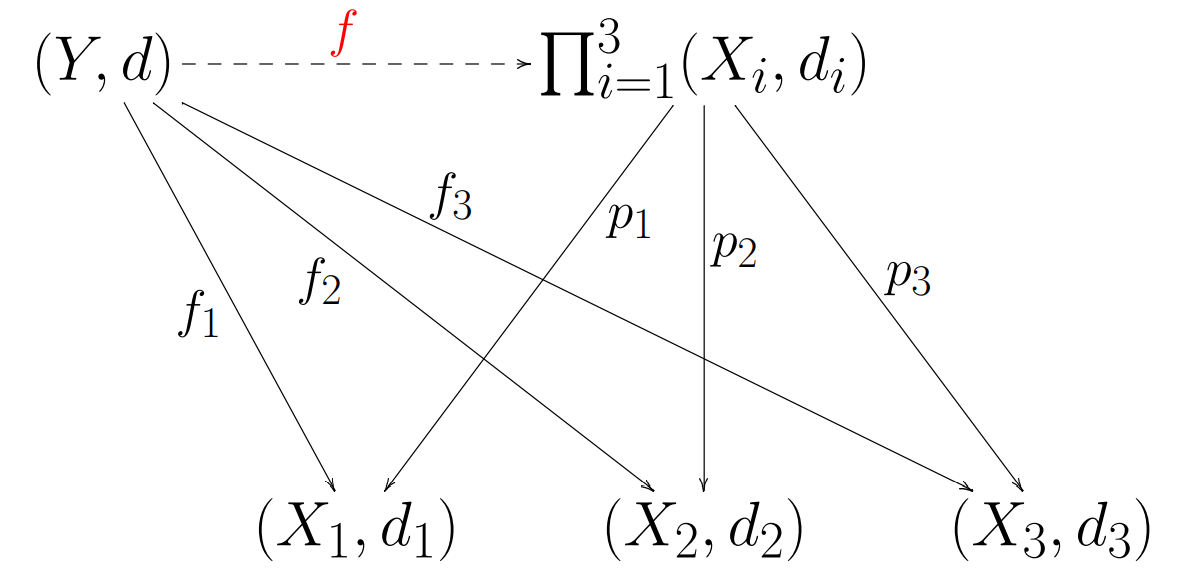
\includegraphics[width=9cm,height=4.8cm]{ipkm.png}
\end{center}
Existuje přesně jedno $f$ takové, že 
\[p_i \circ f = f_i\]
a je spojité.

\noindent

%%%%%%%%%%%%%%%%%%%%%%%%%%%%%%%%%%%%%%%%%%%%%%%%%%%%%%%%%%%%%%%%%%%%%%%%%%%%%%%%%%%%%%%%%%%%%%%%%%%%%%%%%
\section{Parciální derivace}

%%%%%%%%%%%%%%%%%%%%%%%%%%%%%%%%%%%%%%%%%%%%%%%%%%%%%%%%%%%%%%%%%%%%%%%%%%%%%%%%%%%%%%%%%%%%%%%%%%%%%%%%%
\subsection{Definice a značení}
\hspace{1.2mm}
\noindent

\hspace{1.2mm}
Pro $f(x_1,...,x_n)$ vezmeme 
\[\phi_k(t) = f(x_1,...,x_{k-1},t,x_{k+1},...x_n)\]
\[... t = x_k...\]
\hspace{1.2mm}
\textit{Parciální derivace} funkce $f$ podle $x_k$ (v bodě $(x_1,...,x_n))$ je (obvyklá) derivace funkce $\phi_k$,
\[\lim_{h\rightarrow 0}\frac{f(x_1,...,x_{k-1},x_k+h,x_{k+1},...x_n) - f(x_1,..)}{h}.\]
\hspace{1.2mm}
Označení
\[\frac{\partial f(x_1,...(x_n)}{\partial x_k} \textrm{ nebo } \frac{\partial f}{\partial x_k} (x_1,...,x_n),\]
\hspace{1.2mm}
Pro $f(x,y)$ píšeme
\[\frac{\partial f(x,y)}{\partial x} \textrm{ a } \frac{\partial f(x,y)}{\partial y}, \textrm{ atd.}\]

\hspace{1.2mm}
Když $\frac{\partial f(x_1,...,x_n)}{\partial x_k}$ existuje pro všechna $(x_1,...,x_n)$ v nějaké oblasti $D$ máme funkci

\[\frac{\partial f}{\partial x_k}: D \rightarrow \mathbb{R}.\]

\hspace{1.2mm}
Když budeme mluvit o parciální derivaci bude vždy zřejmé máme-li na mysli funkci, nebo jen číslo (hodnotu té limity nahoře).
\noindent

%%%%%%%%%%%%%%%%%%%%%%%%%%%%%%%%%%%%%%%%%%%%%%%%%%%%%%%%%%%%%%%%%%%%%%%%%%%%%%%%%%%%%%%%%%%%%%%%%%%%%%%%%
\subsection{Totální diferenciál}
\hspace{1.2mm}
Nespojitá funkce $f$ může mít po souřadnicích má obě parciální derivace v každém bodě, to však ale neimplikuje spojitost.

\begin{center}
    existence parciálních derivací neimplikuje spojitost!
\end{center}

\hspace{1.2mm}
Budeme potřebovat něco silnejšího. Připomeňte si tvrzení ekvivalentní se standardní derivací:

Existuje $\mu$ konvergujíci k 0 při $h \rightarrow 0$ a A takové, že 

\[f(x+h) - f(x) = Ah + |h| \cdot \mu(h)\]

\hspace{1.2mm}
\textit{Geometrický pohled:}
$f(x+h) - f(x) = Ah$ vyjadřuje tečnu ke grafu funkce v bodě $(x,f(x)).$

\hspace{1.2mm}
$|h|\cdot \mu(h)$ je jakási malá chyba.
\noindent

\hspace{1.2mm}
Mysleme podobně o funkci $f(x,y)$ a uvažujme plochu 
\[S = \{(t,u,f(t,u)) : (t,u) \in D\}.\]

\hspace{1.2mm}
Dvě parciální derivace vyjadřují směry dvou tečných přímek k S vbode $(x,y,f(x,y))$, ale \underline{ne tečnou rovinu}, 
která teprve bude uspokojivé rozšíření faktu nahoře.


\hspace{1.2mm}
Pro \textbf{x} $\in \mathbb{E}_n$ definujeme
\[||\textbf{x}||  = \max_i|x_i|\]

\hspace{1.2mm}
To bude místo absolutní hodnoty, místo $h$ bude $n$-tice blízká nule.
\noindent

%%%%%%%%%%%%%%%%%%%%%%%%%%%%%%%%%%%%%%%%%%%%%%%%%%%%%%%%%%%%%%%%%%%%%%%%%%%%%%%%%%%%%%%%%%%%%%%%%%%%%%%%%
\subsubsection{Definice}
Funkce $f$ má \textit{totální diferenciál} v bodě \textbf{x} existuje-li funkce $\mu$ spojitá v okolí $U$ bodu $o$ taková, že $\mu(\textbf{o}) = 0$
a čísla $A_1,...,A_n$ pro která

\[f(\textbf{a}+\textbf{h}) - f(\textbf{a}) = \sum^n_{k=1}A_kh_k+||\textbf{h}||\mu(\textbf{h}).\]
\hspace{1.2mm}
\noindent

%%%%%%%%%%%%%%%%%%%%%%%%%%%%%%%%%%%%%%%%%%%%%%%%%%%%%%%%%%%%%%%%%%%%%%%%%%%%%%%%%%%%%%%%%%%%%%%%%%%%%%%%%
\subsubsection{Tvrzení o spojitosti funkce a totálním diferenciálu}
\hspace{1.2mm}
Nechť má funkce $f$ totální diferenciál v bodě \textbf{a}. Potom platí, že 
\begin{enumerate}
    \item $f$ je spojitá v \textbf{a},
    \item $f$ má všechny parciální derivace v \textbf{a}, a to s hodnotami 
    
    \[\frac{\partial f(\textbf{a})}{\partial x_k} = A_k.\]
\end{enumerate}
Důkaz:
\begin{enumerate}
    \item Máme
    
    \[|f(\textbf{x}-\textbf{y})| \leq |\textbf{A}(\textbf{x}-\textbf{y})| + |\mu(\textbf{x}-\textbf{y})|\cdot||\textbf{x}-\textbf{y}||\]
    a limita na pravé straně pro \textbf{y} $\rightarrow$ \textbf{x} je 0.
    
    \item Máme 
    \[\frac{1}{h}(f(...x_{k-1},x_k+h,x_{k+1},...) - f(x_1,...)) = A_k + \mu((...,0,h,0,...))\frac{||(0,...,h,...,0)||}{h},\]
    a limita na pravé straně je zřejmě $A_k$.
    
\end{enumerate}
    Teď již spojitost dostaneme. Vidíme, že v případě funkcí jedné proměnné není rozdíl mezi existencí derivace v bodě \textbf{a} a vlastností
    mít totální diferenciál v tomto bodě. V případě více proměnných je však tento rozdíl zcela zásadní. Může být trochu překvapujíci, že 
    zatímco existence parciálních derivací mnoho neznamená, \underline{existence spojitých parciálních derivací} je něco úplně jiného.
\noindent

%%%%%%%%%%%%%%%%%%%%%%%%%%%%%%%%%%%%%%%%%%%%%%%%%%%%%%%%%%%%%%%%%%%%%%%%%%%%%%%%%%%%%%%%%%%%%%%%%%%%%%%%%
\subsubsection{Věta o totálním diferenciálu}
\hspace{1.2mm}
Buď

\[\textbf{h}^{(0)} = \textbf{h}, \textbf{h}^{(1)} = (0, h_2,...,h_n), \textbf{h}^{(2)} = (0,0,h_3,...,h_n) \textrm{ atp.} \]
(takže $\textbf{h}^{(n)} = \textbf{0})$. Potom máme

\[f(\textbf{a}+\textbf{h}) - f(\textbf{a}) = \sum^n_{k=1}(f(\textbf{a}+\textbf{h}^{(k-1)})-f(\textbf{a}+\textbf{h}^{(k)})) = M.\]

Podle Lagrangeovy věty existují $0 \leq \Theta_k \leq 1$ takové, že
\[f(\textbf{a}+\textbf{h}^{(k-1)})-f(\textbf{a}+\textbf{h}^{(k)}) = \frac{\partial f(a_1,...,a_{k-1},a_k+ \theta_kh_k,a_{k+1},...,a_n)}{\partial x_k}h_k\]

a můžeme pokračovat

\begin{align*} 
\begin{split}
M & = \sum\frac{\partial f(a_1,...a_k+\Theta_kh_k,...,a_n)}{\partial x_k}h_k = \\
 & = \sum \frac{\partial f(\textbf{a})}{\partial x_k} + \sum \left( \frac{\partial f(a_1,...,a_k+\Theta_kh_k,...,a_n)}{\partial x_k}
 - \frac{\partial f(\textbf{a})}{\partial x_k} \right)h_k = \\
 & = \sum \frac{\partial f(\textbf{a})}{\partial x_k}h_k + ||\textbf{h}||\sum\left(\frac{\partial f(a_1,...,a_k+\Theta_kh_k,...,a_n)}
 {\partial x_k}- \frac{\partial f(\textbf{a})}{\partial x_k}\right)\frac{h_k}{||\textbf{h}||}.
\end{split}
\end{align*}

Položíme
\[\mu (\textbf{h}) = \sum\left(\frac{\partial f(a_1,...,a_k+\Theta_kh_k,...,a_n)}{\partial x_k} -
    \frac{\partial f(\textbf{a})}{\partial x_k} \right)\frac{h_k}{||\textbf{h}||}.\]
    
    Jelikož $\left|\frac{h_k}{||\textbf{h}||}\right| \leq 1$ a jelikož jsou funkce $\frac{\partial f}{\partial x_k}$ spojité,
    $\lim_{\textbf{h}\rightarrow \textbf{0}} \mu (\textbf{h}) = 0$.
    \begin{center}
    \LARGE 
    Můžeme tedy schematicky psát
    
    \LARGE 
    spojité PD $\implies$ TD $\implies$ PD
    \end{center}
\noindent

%%%%%%%%%%%%%%%%%%%%%%%%%%%%%%%%%%%%%%%%%%%%%%%%%%%%%%%%%%%%%%%%%%%%%%%%%%%%%%%%%%%%%%%%%%%%%%%%%%%%%%%%%
\subsection{Pravidla pro počítání parciálních derivací}
\hspace{1.2mm}
\noindent
Aritmetická pravidla jsou stejná jako pro obyčejné derivace(tady totiž obyčejnými derivacemi jsou).
Trochu jinak tomu je u pravidla pro skládání. Pro derivace jedné proměnné se dokazuje z formule
\[ f(a+h) - f(a) = Ah + |h|\mu (h) \]
tedy z diferenciálu(který je pro ně totéž jako existence derivace). Pravidlo pro skládání v
Pravidlo pro skládání v nejjednodušší podobě následuje.

%%%%%%%%%%%%%%%%%%%%%%%%%%%%%%%%%%%%%%%%%%%%%%%%%%%%%%%%%%%%%%%%%%%%%%%%%%%%%%%%%%%%%%%%%%%%%%%%%%%%%%%%%
\subsubsection{Věta pro derivaci složených funkcí o více proměnných}
\hspace{1.2mm}
Nechť má $f(\textbf{x})$ totální diferenciál v bodu \textbf{a}. Nechť mají $g_k(t)$ derivace v bodě b a nechť je $g_k(b) = a_k$ pro 
$k = 1,...n.$ Položme
\[F(t) = f(\textbf{g}(t)) = f(g_1(t),...g_n(t)).\]

Potom má $F$ derivaci v b, totiž 
\[F'(b) = \sum^n_{k=1}\frac{\partial f(\textbf{a})}{\partial x_k} \cdot g'_k(b).\]

Důkaz:

\begin{align*} 
 \frac{1}{h} (F(b+h) - F(b)) &= \frac{1}{h}(f(\textbf{g}(b+h)) - f(\textbf{g}(b)) =  \\
 &=\frac{1}{h}(f(\textbf{g}(b) + (\textbf{g}(b+h) - \textbf{g}(b))) - f(\textbf{g}(b)) = \\
 &=\sum^n_{k=1}A_k\frac{g_k(b+h)-g_k(b)}{h} + \mu(\textbf{g}(b+h) - \textbf{g}(b)) \max_k\frac{|g_k(b+h)-g_k(b)|}{h}.
\end{align*}

Máme li $lim_{h \rightarrow 0} \mu(\textbf{g}(b+h)-\textbf{g}(b)) = 0$ jelikož jsou funkce $g_k$ spojité v $b$. 
Jelikož funkce $g_k$ mají derivace, jsou $\max_k \frac{|g_k(b+h) - g_k(b)|}{h}$ omezené v dostatečně malém okolí nuly. Limita 
poslední sčítance je tedy nula a máme

\[\lim_{h \rightarrow 0} \frac{1}{h}(F(b+h) - F(b)) = \lim_{h \rightarrow 0} \sum^n_{k = 1} A_k\frac{g_k(b+h)-g_k(b)}{h} = \]
\[= \sum^n_{k = 1}A_k\lim_{h \rightarrow 0} \frac{g_k(b+h) - g_k(b)}{h} = \sum^n_{k = 1}\frac{\partial f(\textbf{a})}{\partial x_k}g'_k(b)\]

\hspace{1.2mm}
Co se děje geometricky: Tečná nadrovina vyjádřená diferenciálem vnější funkce $f$ nemá žádny důvod preferovat hlavní osy v nichž se 
dějí derivace vnitřních funkcí. Proto by tady jen parciálni derivace nestačily. 
\noindent

%%%%%%%%%%%%%%%%%%%%%%%%%%%%%%%%%%%%%%%%%%%%%%%%%%%%%%%%%%%%%%%%%%%%%%%%%%%%%%%%%%%%%%%%%%%%%%%%%%%%%%%%%
\subsubsection{Důsledek (Řetízkové Pravidlo)}
\hspace{1.2mm}
Nechť má $f(\textbf{x})$ \textit{totální diferenciál} v bodě \textbf{a}. Nechť mají funkce $g_k(t_1,...,t_r)$ parciální 
derivace v \textbf{b} $= (b_1,...,b_r)$ a nechť je $g_k(\textbf{b}) = a_k$ pro $k = 1,...,n.$ Potom má funkce
\[(f\circ \textbf{g})(t_1,...,t_r) = f(\textbf{g}(t)) = f(g_1(t),...,g_n(t))\]
všechny parciální derivace v b, a platí 
\[\frac{\partial (f \circ \textbf{g})(\textbf{b})}{\partial t_j} = \sum^n_{k=1}\frac{\partial f(\textbf{a})}{\partial x_k}
\cdot \frac{\partial g_k(\textbf{b})}{\partial t_j}.\]

Skládali jsme

\[\mathbb{E}_k \xrightarrow{\mathbf{g}} \mathbb{E}_n \xrightarrow{\textit{f}} \mathbb{R} \]
Skládejme místo $f$ $m$-tici funkcí
$\mathbf{f} = (f_1,...,f_m)$, tedy $\mathbf{f}: \mathbb{E}_n \rightarrow \mathbb{E}_M$
\[\mathbb{E}_k \xrightarrow{\mathbf{g}} \mathbb{E}_n \xrightarrow{\textit{f}} \mathbb{E}_m \]
Pravidlo z předchozí věty dá tedy
\[\frac{\partial (f_i \circ \mathbf{g})(b)}{\partial t_j} = \sum^n_{k=1} \frac{\partial f_i(\mathbf{a})}{\partial x_k}
\cdot \frac{\partial g_k(\mathbf{b})}{\partial t_j}.\]

Zavedeme-li matice $D\mathbf{f} = \left(\frac{\partial f_i(\mathbf{a}}{\partial x_k}\right)_{ik}$ je 
$D(\mathbf{f}\circ \mathbf{g} = D\mathbf{f}\cdot D\mathbf{g}$ (napravo násobení matic), a tak to má být. $D\mathbf{h}$ je matice lineární aproximace 
funkce $\mathbf{h}$: \textit{lineární aproximace se skládají spolu s aproximovanými funkcemi}.
\noindent

%%%%%%%%%%%%%%%%%%%%%%%%%%%%%%%%%%%%%%%%%%%%%%%%%%%%%%%%%%%%%%%%%%%%%%%%%%%%%%%%%%%%%%%%%%%%%%%%%%%%%%%%%
\subsection{Aritmetická pravidla z řetězového násobení}
%%%%%%%%%%%%%%%%%%%%%%%%%%%%%%%%%%%%%%%%%%%%%%%%%%%%%%%%%%%%%%%%%%%%%%%%%%%%%%%%%%%%%%%%%%%%%%%%%%%%%%%%%
\subsubsection{Násobení}
\[ f(u,v) = u \cdot v \]

\hspace{1.2mm}
\noindent
Potom $ \frac{\partial f}{\partial u} = v $ a $ \frac{\partial f}{\partial v} = u $
a pro $u = \psi (x)$ a $ v = \phi (x) $ platí:
\[ (\phi (x), \psi (y))' =
\frac{\partial f}{\partial u} \phi '(x) + \frac{\partial f}{\partial v} \psi '(x) = 
\phi (x)\psi '(x) + \phi '(x)\psi (x)  \]

%%%%%%%%%%%%%%%%%%%%%%%%%%%%%%%%%%%%%%%%%%%%%%%%%%%%%%%%%%%%%%%%%%%%%%%%%%%%%%%%%%%%%%%%%%%%%%%%%%%%%%%%%%
\subsubsection{Dělení}
\[ f(u,v) = \frac{u}{v} \]

\hspace{1.2mm}
\noindent
Potom $ \frac{\partial f}{\partial u} = \frac{1}{v} $ a $ \frac{\partial f}{\partial v} = -\frac{u}{v^2} $
a pro $u = \psi (x)$ a $ v = \phi (x) $ platí:
\[ \left( \frac{\phi (x)}{\psi (x)} \right)' =
\frac{\partial f}{\partial u} \phi '(x) - \frac{\partial f}{\partial v} = \psi '(x) =
\frac{1}{\psi (x)} \phi '(x) + \frac{1}{\psi (x)^2}\psi '(x) =
\frac{\psi (x)\phi '(x) - \phi (x)\psi '(x)}{\psi (x)^2} \]

\subsection{Lagrangeova věta ve více proměnných}
%-> možno by bolo dobré doplniť aj vetou pre jednu premennú
\hspace{1.2mm}
\noindent
Nechť má $f$ spojité parciální derivace v konvexní otevřené množině $U \subseteq \mathbb{E}_{n}$.
Potom pro libovolné dva body $x,y \in D \exists 0 \leq \theta \leq 1$ takové, že:
\[ f(\mathbf{y}) - f(\mathbf{x}) =
\sum^{n}_{j=1} \frac{\partial f(\mathbf{x} + \theta (\mathbf{y}-\mathbf{x}))}{\partial x_j}(y_j - x_j) \]

\noindent
\textbf{Důkaz:}
Mějme $\mathbf{g}$, pro které platí $g_j(t) = x_j + t(y_j - x_j)$.
Potom máme $F(t) = f \circ \mathbf{g} = (\mathbf{x} + t(\mathbf{y}-\mathbf{x}))$ a
\[ F'(t) = \sum^{n}_{j=1} \frac{\partial f(\mathbf{g}(t))}{\partial x_j}g_j'(t) =
\sum^{n}_{j=1} \frac{\partial f(\mathbf{g}(t))}{\partial x_j}(y_j - x_j)  \]
Podle Lagrangeovy věty:
\[ f(\mathbf{y}) - f(\mathbf{x}) = F(1) - F(0) = F'(\theta) \]

\noindent
\textbf{Poznámka:}
Často se užívá v tomto tvaru:
\[ f(\mathbf{x} + \mathbf{h}) - f(\mathbf{x}) =
\sum^{n}_{j=1} \frac{\partial f(\mathbf{x + \theta \mathbf{h}})}{\partial x_j}h_j \]
(Porovnej s formulí pro totální diferenciál)
%%%%%%%%%%%%%%%%%%%%%%%%%%%%%%%%%%%%%%%%%%%%%%%%%%%%%%%%%%%%%%%%%%%%%%%%%%%%%%%%%%%%%%%%%%%%%%%%%%%%%%%%%

\subsection{Tvrzení o záměnnosti pořadí při parciálních derivacích}
\hspace{1.2mm}
\noindent
Mějme funkci $f(x,y)$ takovou, že existují parciální derivace
$\frac{\partial ^2 f}{\partial x \partial y}$ a $\frac{\partial ^2 f}{\partial y \partial x}$, které
jsou spojité v nějakém okolí bodu $(x,y)$. Potom:
\[ \frac{\partial ^2 f(x,y)}{\partial x \partial y} = \frac{\partial ^2 f(x,y)}{\partial y \partial x} \]

\noindent
\textbf{Důkaz:} Pokusíme se spočíst obě derivace v jednom kroku, tedy počítejme limitu $lim_{h\rightarrow 0} F(h)$ funkce
\[F(h) = \frac{f(x+h,y+h) - f(x,y+h) - f(x+h,y) + f(x,y)}{h^2}\]
Položíme li 

\begin{align*} 
\begin{split}
\varphi_h(y) & = f(x+h,y) - f(x,y)\text{ a}\\
\psi_k(x) & = f(x,y+k) - f(x,y),
\end{split}
\end{align*}
dostaneme pro $F(h)$ dva výrazy:
\begin{align*} 
\begin{split}
F(h) & = \frac{1}{h^2} (\varphi_h(y+h) - \varphi_h(y))\\
F(h) & = \frac{1}{h^2} (\psi_h(x+h)-\psi_h(x)).
\end{split}
\end{align*}

První: Funkce $\varphi_h$ má derivaci (podle $y$, jinou proměnnou nemá)
\[\varphi'_h(y)=\frac{\partial f(x+h,y)}{\partial y}-\frac{\partial f(x,y)}{\partial y}\]

a tedy podle Lagrangeovy formule
\begin{align*}
    F(h) & = \frac{1}{h^2}(\varphi_h(y+h)-\varphi_h(y)) = \frac{1}{h}\varphi'_h(y+\theta_1h)\\
    & = \frac{\partial f(x+h,y+\theta_1h)}{\partial y} -\frac{\partial f(x,y+\theta_1h)}{\partial y}.
\end{align*}

Potom znovu, podle L. formule,
\[F(h) = \frac{\partial }{\partial x}\left(\frac{\partial f(x+\theta_2h,y+\theta_1h}{\partial y}\right)\]

pro nějaká $\theta_1,\theta_2$ mezi 0 a 1.

Druhá, $\frac{1}{h^2}(\varphi_h(x+h) - \varphi_h(x)))$ dá podobně
\[F(h) = \frac{\partial }{\partial y}\left(\frac{\partial f(x+\theta_4h,y + \theta_2h}{\partial x}\right)\]
Obě $\frac{\partial }{\partial y}(\frac{\partial f}{\partial x})$ a $\frac{\partial }{\partial x}(\frac{\partial f}{\partial y})$ jsou spojité ($x,y$), a $lim_{h\rightarrow 0} F(h)$ můžeme počítat z kteréhokoli výrazu (první nebo druhá):

\[\lim_{h\rightarrow 0}F(h) = \frac{\partial ^2 f(x,y)}{\partial x \partial y} 
                            = \frac{\partial ^2 f(x,y)}{\partial y \partial x}.\]
%%%%%%%%%%%%%%%%%%%%%%%%%%%%%%%%%%%%%%%%%%%%%%%%%%%%%%%%%%%%%%%%%%%%%%%%%%%%%%%%%%%%%%%%%%%%%%%%%%%%%%%%%
\subsubsection{Důsledek tvrzení o záměnnosti}
\hspace{1.2mm}
Nechť má funkce $f$ v proměnných spojité parciální derivace do řádu $k$. Potom hodnoty těchto derivací
záleží pouze na tom, kolikrát bylo derivováno v každé z proměnných $x_1, ... , x_n$.

\noindent
\hspace{1.2mm}
Tedy za daných předpokladů můžeme obecné parciální derivace řádu $r \leq k$ psát
\[\frac{\partial ^r f}{\partial x^{r_1}_1 \partial x^{r_2}_2 ... \partial x_n^{r_n}} \text{ kde } r_1 + r_2 + \cdot \cdot \cdot + r_n = r \]
\[(r_j = 0 \text{ indukuje absenci symbolu } \partial x_j)\]

%%%%%%%%%%%%%%%%%%%%%%%%%%%%%%%%%%%%%%%%%%%%%%%%%%%%%%%%%%%%%%%%%%%%%%%%%%%%%%%%%%%%%%%%%%%%%%%%%%%%%%%%%
\subsection{Věta o konvergentní podposloupnosti}
\hspace{1.2mm}
\noindent
Z každé posloupnosti na kompaktním intervalu lze vybrat konvergentní podposloupnost.

\noindent
\hspace{1.2mm}
Explicitně:
Mějme $a,b \in \mathbb{R}$ taková, že $\forall n: a \leq x_n \leq b$. Potom existuje podposloupnost
$(x_{k_n})_n$ posloupnosti $(x_n)_n$ která konverguje v $\mathbb{R}$ a platí
$a \leq \lim_n x_{k_n} \leq b$

\vspace{5mm}
\noindent
\textbf{Důkaz:} 
Vezměme \[M = \{x : x \in \mathbb{R}, x \leq x_n \text{ pro nekonečně mnoho n}\}\]
$M$ je neprázdná a omezená protože $a \in M \text{ a } b$ je horní mez $M$. Musí tedy existovat $s = sup(M)$ a platí 
$a \leq s \leq b$. Dále, pro každé $n$ je množina 
\[K(n) = \{k : s - \frac{1}{n} < x_k < s + \frac{1}{n}\}\]
nekonečná: skutečně, máme $x > s - \varepsilon$ takové, že $x_n > x$ pro nekonečně mnoho $n$, zatím co podle definice množiny M je jen
konečně mnoho $n$ takových, že $x_n \geq s + \varepsilon$. 

Zvolme $k_1$ tak, aby
\[s - 1 < x_{k_{1_2}} < s+1.\]
Mějme zvolena $k_1 < k_2 < \cdot \cdot \cdot < k_n$ taková, že $j = 1,...,n$
\[s - \frac{1}{j} < x_{k_j} < s + \frac{1}{j}.\]
Jelikož $K(n+1)$ je nekonečná, můžeme zvolit $k_{n+1} > k_n$ tak, aby
\[s - \frac{1}{n+1} < x_{k_{n+1}} < s + \frac{1}{n+1}.\]
Takto zvolená podposloupnost $(x_{k_n})_n$ naší $(x_n)_n$ zřejmě konverguje k $s$.

%%%%%%%%%%%%%%%%%%%%%%%%%%%%%%%%%%%%%%%%%%%%%%%%%%%%%%%%%%%%%%%%%%%%%%%%%%%%%%%%%%%%%%%%%%%%%%%%%%%%%%%%%
\section{Kompaktní prostory}
%%%%%%%%%%%%%%%%%%%%%%%%%%%%%%%%%%%%%%%%%%%%%%%%%%%%%%%%%%%%%%%%%%%%%%%%%%%%%%%%%%%%%%%%%%%%%%%%%%%%%%%%%
\subsection{Definice kompaktního prostoru}
\hspace{1.2mm}
\noindent
Metrický prostor $(X,d)$ je kompaktní, pokud každá posloupnost v něm obsahuje konvergentní podposloupnost.

%%%%%%%%%%%%%%%%%%%%%%%%%%%%%%%%%%%%%%%%%%%%%%%%%%%%%%%%%%%%%%%%%%%%%%%%%%%%%%%%%%%%%%%%%%%%%%%%%%%%%%%%%
\newpage
\subsection{Tvrzení o podprostoru kompaktního prostoru}
\hspace{1.2mm}
\noindent
Podprostor kompaktního prostoru je kompaktní právě když je uzavřený.

\vspace{5mm}
\noindent
\textbf{Důkaz:} 
\begin{enumerate}
    \item Buď $Y$ uzavřený podprostor kompaktního $X$ a buď $(y_n)_n$ podposloupnost v $Y$. Jako posloupnost v X má podposloupnost s limitou
    a z uzavřenosti je tato limita v $Y$.
    \item Nechť $Y$ není uzavřená. Potom existuje posloupnost $(y_n)_n)$ v $Y$ konvergentní v $X$ taková, že $y = lim_n y_n \notin Y$. Potom $(y_n)_n$
    nemůže mít podposloupnost konvergentní v $Y$ protože každá její podposloupnost konverguje k $y$.
\end{enumerate}

%%%%%%%%%%%%%%%%%%%%%%%%%%%%%%%%%%%%%%%%%%%%%%%%%%%%%%%%%%%%%%%%%%%%%%%%%%%%%%%%%%%%%%%%%%%%%%%%%%%%%%%%%
\subsection{Tvrzení o uzavřenosti podprostoru}
\hspace{1.2mm}
\noindent
Buď $(X,d)$ libovolný metrický prostor a
buď podprostor $Y \subseteq X$ kompaktní. Potom $Y$ je uzavřený v $(X,d)$.

\vspace{5mm}
\noindent
\textbf{Důkaz:} Nechť $(y_n)_n$ posloupnost v $Y$ konverguje v $X$ k limitě $y$. Potom každá podposloupnost $(y_n)_n$ konverguje k 
$y$ a tedy je $y \in Y$.
\begin{center}
    Metrický prostor $(X,d)$ je omezený, jestliže pro nějaké $K$ platí, že 
    \[\forall x,y \in X : d(x,y) < K.\]
\end{center}

%%%%%%%%%%%%%%%%%%%%%%%%%%%%%%%%%%%%%%%%%%%%%%%%%%%%%%%%%%%%%%%%%%%%%%%%%%%%%%%%%%%%%%%%%%%%%%%%%%%%%%%%%
\subsection{Tvrzení o omezenosti kompaktního prostoru}
\hspace{1.2mm}
\noindent
Každý kompaktní prostor je omezený.

\vspace{5mm}
\noindent
\textbf{Důkaz:} Zvolme $x_1$ libovolně a $x_n$ tak, aby $d(x_1,x_n) > n$. Posloupnost $(x_n)_n$ nemá konvergentní podposloupnost; kdyby $x$
byla limita takové podposloupnosti, bylo by pro dost velké $n$ nekonečně mnoho členů této podposloupnosti blíže k $x_1$ než $d(x_1,x_n)+1$, což je spor.

%%%%%%%%%%%%%%%%%%%%%%%%%%%%%%%%%%%%%%%%%%%%%%%%%%%%%%%%%%%%%%%%%%%%%%%%%%%%%%%%%%%%%%%%%%%%%%%%%%%%%%%%%
\subsection{Věta o součinu kompaktních prostorů}
\hspace{1.2mm}
\noindent
Součin konečně mnoha kompaktních prostorů je kompaktní.

\vspace{5mm}
\noindent
\textbf{Důkaz:} Stačí dokázat pro součin dvou prostorů.

Buďte $(X,d_1), (X, d_2)$ kompaktní a buď $((x_n,y_n))_n$ posloupnost v $X \times Y$. 
Zvolme konvergentní podposloupnost $(x_{k_n})_n$ posloupnosti $(x_n)_n$ a konvergentní podposloupnost $(y_{k_{l_n}})_n$ posloupnosti $(y_{k_n})_n$.

Potom je 
\[((x_{k_{l_n}},y_{k_{l_n}}))_n\]
konvergentní podposloupnost posloupnosti $((x_n,y_n))_n$.

\begin{center}
    Kompaktní interval v $\mathbb{E}_n$: součin intervalů $\left<a_i,b_i\right>$
\end{center}

%%%%%%%%%%%%%%%%%%%%%%%%%%%%%%%%%%%%%%%%%%%%%%%%%%%%%%%%%%%%%%%%%%%%%%%%%%%%%%%%%%%%%%%%%%%%%%%%%%%%%%%%%
\newpage
\subsection{Věta : podprostor euklidovského prostoru je kompaktní právě když je omezený a uzavřený}
\hspace{1.2mm}
\noindent
Podprostor euklidovského prostoru $\mathbb{E}_n$ je kompaktní právě když je uzavřený a omezený.

\vspace{5mm}
\noindent
\textbf{Důkaz:} 
\begin{enumerate}
    \item Že je uzavřený a omezený už víme.
    \item Buď nyní $Y \subseteq \mathbb{E}_n$ omezený a uzavřený. Jelikož je omezený, je pro dostatečně velký kompaktní interval
    \[Y \subseteq J^n \subseteq \mathbb{E}_n.\]
    $J^n$ je kompaktní jako součin intervalů $\left<a_i,b_i\right>$, a jelikož je $Y$ uzavřený v $\mathbb{E}_n$ je též uzavřený
    v $J^n$ a tedy kompaktní.
\end{enumerate}

%%%%%%%%%%%%%%%%%%%%%%%%%%%%%%%%%%%%%%%%%%%%%%%%%%%%%%%%%%%%%%%%%%%%%%%%%%%%%%%%%%%%%%%%%%%%%%%%%%%%%%%%%
\subsection{Tvrzení: obraz spojitého zobrazení je kompaktní}
\hspace{1.2mm}
\noindent
Buď $f: (X,d) \to (Y, d')$ spojité zobrazení a buď $A \subseteq X$ kompaktní. Potom je $f[A]$ kompaktní.


\vspace{5mm}
\noindent
\textbf{Důkaz:} Buď $(y_n)_n$ posloupnost v $f[A]$. Zvolme $x_n \in A$ tak, aby $y_n = f(x_n)$. Buď $(x_{k_n})_n$ konvergentní podposloupnost
Potom je $(y_{k_n})_n = (f(x_{k_n}))_n$ konvergentní podposloupnost $(x_n)_n$.

%%%%%%%%%%%%%%%%%%%%%%%%%%%%%%%%%%%%%%%%%%%%%%%%%%%%%%%%%%%%%%%%%%%%%%%%%%%%%%%%%%%%%%%%%%%%%%%%%%%%%%%%%
\subsection{Tvrzení: každá spojitá funkce na kompaktním prostoru nabýva maxima i minima}
\hspace{1.2mm}
\noindent
Buď $(X,d)$ kompaktní. Potom každá spojitá funkce $f:(X,d)\to \mathbb{R}$ nabývá maxima i minima.

\vspace{5mm}
\noindent
\textbf{Důkaz:} Buď $Y = f[X] \subseteq \mathbb{R}$ kompaktní. Je to tedy omezená množina a musí mít supremum $M$ a infimum $m$. Zřejmě máme 
$d(m,Y) = d(M,Y) = 0$ a jelikož $Y$ je uzavřená, $m,M \in Y$. Víme, že spojitá $f$ je charakterizována tím, že všechny vzory uzavřených množin
jsou uzavřené. Nyní vidíme, že je-li definiční obor kompaktní, platí též, že obrazy uzavřených podmnožin jsou uzavřené. Z toho plyne následujíci:

%%%%%%%%%%%%%%%%%%%%%%%%%%%%%%%%%%%%%%%%%%%%%%%%%%%%%%%%%%%%%%%%%%%%%%%%%%%%%%%%%%%%%%%%%%%%%%%%%%%%%%%%%
\subsection{Věta o vzájemně jednoznačném spojitém zobrazení}
\hspace{1.2mm}
\noindent
Je-li $(X,d)$ kompaktní a je-li $f: (X,d) \to (Y,d')$ vzájemně jednoznačné spojité zobrazení, pak je
$f$ homeomorfismus.

\vspace{2mm}
\hspace{1.2mm}
{\small
Obecněji: Nechť $f:(X,d) \to (Y,d')$ je spojité zobrazení. Mějme potom $g: (X,d) \to (Z, d'')$ a
$h: (Y,d') \to (Z,d'')$ takové, že $h \circ f = g$. Potom je $h$ spojité.}

\vspace{5mm}
\noindent
\textbf{Důkaz:} Buď $B$ uzavřená v $Z$. Potom je $A = g^{-1}[B]$ uzavřená $\implies$ kompaktnost v $X$ $\implies$ $f[A]$ je kompaktní $\implies$ uzavřená v $Y$. Jelikož  je $f$ zobrazení na, máme $f[f^{-1}[C]] = C \forall C$. Proto je 
\[h^{-1}[B] = f[f^{-1}[h^{-1}[B]]] = f[(h \circ f)^{-1}[B]] = f[g^{-1}[B]] = f[A]\]
uzavřená.

%%%%%%%%%%%%%%%%%%%%%%%%%%%%%%%%%%%%%%%%%%%%%%%%%%%%%%%%%%%%%%%%%%%%%%%%%%%%%%%%%%%%%%%%%%%%%%%%%%%%%%%%%
\subsection{Definice cauchyovské posloupnosti $(x_n)_n$}
\hspace{1.2mm}
\noindent
Posloupnost $(x_n)_n$ v $(X,d)$ je \textbf{Cauchyovská}, jestliže
\[ \forall \epsilon > 0 \exists n_0: m,n \geq n_0 \implies d(x_m, x_n) < \epsilon \]

%%%%%%%%%%%%%%%%%%%%%%%%%%%%%%%%%%%%%%%%%%%%%%%%%%%%%%%%%%%%%%%%%%%%%%%%%%%%%%%%%%%%%%%%%%%%%%%%%%%%%%%%%
\subsection{Tvrzení o konvergenci cauchyovské posloupnosti}
\hspace{1.2mm}
\noindent
Nechť má Cauchyovská posloupnost konvergentní podposloupnost. Potom posloupnost konverguje k limitě
podposloupnosti.

\vspace{5mm}
\noindent
\textbf{Důkaz:} Nechť je $(x_n)_n$ Cauchyovská a nechť $lim_{n}x_{k_n} = x.$ Buď $d(x_m,x_n) < \varepsilon$ pro $m,n \geq n_1$ 
a $d(x_{k_n},x) \leq \varepsilon$ pro $n \geq n_2$. Položíme-li $n_0 = max(n_1,n_2)$, máme pro $n \geq n_0$ (protože $k_n \geq n$)
\[d(x_n,x) \leq d(x_n,x_{k_n}) + d(x_{k_n},x) < 2\varepsilon.\]

%%%%%%%%%%%%%%%%%%%%%%%%%%%%%%%%%%%%%%%%%%%%%%%%%%%%%%%%%%%%%%%%%%%%%%%%%%%%%%%%%%%%%%%%%%%%%%%%%%%%%%%%%
\subsection{Definice úplného metrického prostoru}
\hspace{1.2mm}
\noindent
Metrický prostor $(X,d)$ je \textbf{úplný}, pokud v něm každá Cauchyovská posloupnost konverguje.

%%%%%%%%%%%%%%%%%%%%%%%%%%%%%%%%%%%%%%%%%%%%%%%%%%%%%%%%%%%%%%%%%%%%%%%%%%%%%%%%%%%%%%%%%%%%%%%%%%%%%%%%%
\subsection{Tvrzení: Podprostor úplného prostoru je úplný právě když je uzavřený}
\hspace{1.2mm}
\noindent
Podprostor úplného je úplný, právě když je uzavřený.

\vspace{5mm}
\noindent
\textbf{Důkaz:} 
\begin{enumerate}
    \item Buď $Y \subseteq (X,d)$ uzavřený. Buď $(y_n)_n$ Cauchyovská v $Y$. Potom je Cauchyovská 
    a tedy konvergentní v $X$ a kvůli uzavřenosti je limita v $Y$.
    \item Nechť $Y$ není uzavřený. Potom existuje posloupnost $(y_n)_n$ v $Y$ konvergentní v $X$ taková, že $lim_n y_n \notin Y$.
    Potom je $(y_n)_n$ Cauchyovská v $X$ a jelikož je vzálenost stejná, též v $Y$. Ale v $Y$ nekonverguje.
\end{enumerate}

%%%%%%%%%%%%%%%%%%%%%%%%%%%%%%%%%%%%%%%%%%%%%%%%%%%%%%%%%%%%%%%%%%%%%%%%%%%%%%%%%%%%%%%%%%%%%%%%%%%%%%%%%
\subsection{Tvrzení: Každý kompaktní prostor je úplný}
\hspace{1.2mm}
\noindent
Každý kompaktní prostor je úplný.

\vspace{5mm}
\noindent
\textbf{Důkaz:} Cauchyovská posloupnost má podle kompaktnosti konvergentní podposloupnost a tedy konverguje.

%%%%%%%%%%%%%%%%%%%%%%%%%%%%%%%%%%%%%%%%%%%%%%%%%%%%%%%%%%%%%%%%%%%%%%%%%%%%%%%%%%%%%%%%%%%%%%%%%%%%%%%%%
\subsection{Lemma o cauchyovské posloupnosti}
\hspace{1.2mm}
\noindent
Posloupnost $(x_{1}^{1}, ... , x_{1}^{n}), (x_{1}^{2},...,x_{n}^{2}), ...,(x_{1}^{k},...,x_{n}^{k}),...$
je Cauchyovská v $\prod_{i=1}^{n}(X_i, d_i)$ právě když každá z posloupností $(x_{i}^{k})_k$ je
Cauchyovská v $(X_i, d_i)$.

\vspace{5mm}
\noindent
\textbf{Důkaz:} $\implies$ plyne bezprostředně z toho, že $d_i(u_i,v_i) \leq d((u_j)_j,(v_j)_j).$

$\Leftarrow$: Nechť je každá $(x_i^k)_k$ Cauchyovská. Pro $\varepsilon > 0$ a $i$ zvolme $k_i$ tak,
aby pro $k,l \geq k_i$ bylo $d_i(x_i^k, x_i^l) < \varepsilon.$ Potom pro $k,l \geq$ $\text{max}_i k_i$ máme 
\[d((x_1^k,...,x_n^k),(x_1^l,...,x_n^l)) < \varepsilon.\]

%%%%%%%%%%%%%%%%%%%%%%%%%%%%%%%%%%%%%%%%%%%%%%%%%%%%%%%%%%%%%%%%%%%%%%%%%%%%%%%%%%%%%%%%%%%%%%%%%%%%%%%%%
\subsection{Věta: Součin úplných prostorů je úplný }
\hspace{1.2mm}
\noindent
Součin úplných prostorů je úplný. Speciálně, $\mathbb{E}_n$ je úplný.

\subsubsection{Důsledek}
\hspace{1.2mm}
\noindent
Podprostor $Y$ euklidovského prostoru $\mathbb{E}_n$ je úplný, právě když je uzavřený.

%%%%%%%%%%%%%%%%%%%%%%%%%%%%%%%%%%%%%%%%%%%%%%%%%%%%%%%%%%%%%%%%%%%%%%%%%%%%%%%%%%%%%%%%%%%%%%%%%%%%%%%%%
\section{Implicitní funkce}
\hspace{1.2mm}
\noindent

%%%%%%%%%%%%%%%%%%%%%%%%%%%%%%%%%%%%%%%%%%%%%%%%%%%%%%%%%%%%%%%%%%%%%%%%%%%%%%%%%%%%%%%%%%%%%%%%%%%%%%%%%
\subsection{Ilustrační příklady}

\subsubsection{Obecný příklad}
\noindent
\hspace{1.2mm}
Mějme spojité reálné funkce $F_i(x_1, ... , x_m, y_1, ... , y_n)$ pro každé $i \in \{1, ..., n\}$
v $n + m$
proměnných. Určuje systém rovnic
\[ F_1(x_1, ... , x_m, y_1, ... , y_n) = 0 \]
\[ \vdots \hspace{15mm} \vdots \hspace{15mm} \vdots \]
\[ F_n(x_1, ... , x_m, y_1, ... , y_n) = 0 \]
v nějakém smyslu funkce
\[ f_i \equiv y_i(x_1, ... , x_m) \]
pro $i \in \{ 1, ... , n \}$? Pokud ano, jak a kde je určuje a jaké mají funkce vlastnosti?

\vspace{5mm}
\noindent
\hspace{1.2mm}
Konkrétněji viz následující příklad.

\subsubsection{Příklad pro $F(x,y) = x^2 + y^2 - 1$}
\noindent
\hspace{1.2mm}
Mějme $F(x,y) = x^2 + y^2 - 1$, neboli rovnici \[ x^2 + y^2 = 1 \]

\noindent
\hspace{1.2mm}
Několik pozorování:
\begin{itemize}
    \item Pro některá $x_0$ jako například $x_0 < -1$ řešení neexistuje, o funkci $y(x)$ nemluvě.
    \item Přestože řešení v nějakém okolí $x_0$ existuje, nemůžeme v nějakých situacích hovořit o funkci.
    Potřebujeme kolem řešení $(x_0, y_0)$ vymezit okolí jak $x_0$, tak $y_0$.
    \item Máme také případy, jako ten, kdy $x_0 = 1$, kde je v okolí mnoho řešení, ale žádný(ani
    jednostranný) interval, kde by $y$ bylo jednoznačné.
\end{itemize}

\noindent
\hspace{1.2mm}
V případě $F(x,y)$ už zádná další situace nenastane.

%%%%%%%%%%%%%%%%%%%%%%%%%%%%%%%%%%%%%%%%%%%%%%%%%%%%%%%%%%%%%%%%%%%%%%%%%%%%%%%%%%%%%%%%%%%%%%%%%%%%%%%%%
\subsection{Věta o implicitní funkci}
\hspace{1.2mm}
\noindent
Buď $F(x,y)$ reálná funkce definovaná v nějakém okolí bodu $(x_0, y_0)$. Nechť má $F$ spojité parciální
derivace do řádu $k \geq 1$ a nechť platí:
\begin{align*}
    F(x_0, y_0) &= 0\\
    \left| \frac{\partial F(x_0,y_0)}{\partial y} \right| &\neq 0
\end{align*}
Potom $ \exists \delta > 0$ a $\Delta > 0$ takové, že
$\forall x \in (x_0 - \delta , x_0 + \delta) \exists! y \in (y_0 - \Delta , y_0 + \Delta): F(x,y) = 0$.

\noindent
Dále, označíme-li toto jediné $y$ jako $y = f(x)$, potom získaná
$f: (x_0 - \delta , x_0 + \delta ) \to \mathbb{R}$ má spojité derivace do řádu $k$.

%%%%%%%%%%%%%%%%%%%%%%%%%%%%%%%%%%%%%%%%%%%%%%%%%%%%%%%%%%%%%%%%%%%%%%%%%%%%%%%%%%%%%%%%%%%%%%%%%%%%%%%%%
% Tohle tam psat nebudu, neni to uplne necessary a neukaze ti to nic uplne novyho
%\subsection{Definice (implicitní?) funkce a vlastnosti}
%\hspace{1.2mm}
%(5. str 7)
%\noindent

%%%%%%%%%%%%%%%%%%%%%%%%%%%%%%%%%%%%%%%%%%%%%%%%%%%%%%%%%%%%%%%%%%%%%%%%%%%%%%%%%%%%%%%%%%%%%%%%%%%%%%%%%
\subsection{Věta o implicitních funkcích}
\hspace{1.2mm}
\noindent
Buďte $F_i(\mathbf{x}, y_1, ... , y_m)$ pro $i \in {1, ... , m}$ funkce $n+m$ proměnných se spojitými
parciálními derivacemi do řádu $k \geq 1$. Buď \[ \mathbf{F}(\mathbf{x}^0, \mathbf{y}^0) = \mathbf{o} \]
a \[ \frac{D(\mathbf{F})}{D(\mathbf{y})}(\mathbf{x}^0, \mathbf{y}^0) \neq 0 \]
Potom existují $\delta > 0$ a $\Delta > 0$ takové, že pro každé
\[ \mathbf{x} \in (x_{1}^{0} - \delta, x_{1}^{0} + \delta) \times \cdot \cdot \cdot \times 
(x_{n}^{0} - \delta, x_{n}^{0} + \delta)\]
existuje právě jedno
\[ \mathbf{y} \in (y_{1}^{0} - \Delta , y_{1}^{0} + \Delta) \times \cdot \cdot \cdot \times
(y_{m}^{0} - \Delta , y_{m}^{0} + \Delta) \]
takové, že
\[ \mathbf{F}(\mathbf{x}, \mathbf{y}) = 0 \]

%%%%%%%%%%%%%%%%%%%%%%%%%%%%%%%%%%%%%%%%%%%%%%%%%%%%%%%%%%%%%%%%%%%%%%%%%%%%%%%%%%%%%%%%%%%%%%%%%%%%%%%%%
\subsection{Definice Jacobiho determinantu}
\hspace{1.2mm}
\noindent
Pro konečnou posloupnost funkcí
\[ \mathbf{F}(\mathbf{x}, \mathbf{y}) =
(F_1(\mathbf{x}, y_1, ..., y_m), ... , F_m(\mathbf{x}, y_1, ..., y_m)) \]
a pro $\mathbf{y} = (y_1, ... , y_m)$ se definuje \textbf{Jacobiho determinant}(Jacobián) jako
\[ \frac{D(\mathbf{F})}{D(\mathbf{y})} =
\det \left( \frac{\partial F_i}{\partial y_j} \right)_{i,j \in \{ 1, ... , m\}} \]

%%%%%%%%%%%%%%%%%%%%%%%%%%%%%%%%%%%%%%%%%%%%%%%%%%%%%%%%%%%%%%%%%%%%%%%%%%%%%%%%%%%%%%%%%%%%%%%%%%%%%%%%%
\section{Extrémy}
\hspace{1.2mm}
\noindent

%%%%%%%%%%%%%%%%%%%%%%%%%%%%%%%%%%%%%%%%%%%%%%%%%%%%%%%%%%%%%%%%%%%%%%%%%%%%%%%%%%%%%%%%%%%%%%%%%%%%%%%%%
\subsection{Věta o hledání extrémů funkcí}
\hspace{1.2mm}
\noindent
Buďte $f,g_1, ... , g_k$ reálné funkce definované na otevřené množině $D \subseteq \mathbb{E}_n$.
Nechť mají spojité parciální derivace. Nechť je hodnost matice
\[ M = \begin{pmatrix}
\frac{\partial g_1}{\partial x_1} & \dots & \frac{\partial g_1}{\partial x_n}\\
\vdots & \ddots & \vdots\\
\frac{\partial g_k}{\partial x_1} & \dots & \frac{\partial g_k}{\partial x_n}\\
\end{pmatrix}\]
maximální, tedy $k$, v každém bodě oboru $D$.

\noindent
\hspace{1.2mm}
Jestliže funkce $f$ nabývá v bodě $\mathbf{a} = (a_1, ... , a_n)$ lokálního extrému podmíněného vazbami
\[ g_i(x_1, ... , x_n) = 0 \forall i \in \{ 1, ... , k \} \]
pak existují čísla $\lambda _1, ... , \lambda _k$ taková, že $\forall i \in {1, ... , n}$ platí
\[ \frac{\partial f(\mathbf{a})}{\partial x_i} +
\sum_{j=1}^{k}\lambda_j \cdot \frac{\partial g_j(\mathbf{a})}{\partial x_i} = 0 \]

\vspace{5mm}
\noindent
\textbf{Důkaz:} Matice $M$ má hodnost $k$ právě když aspoň jedna její $k\times k$ podmatice $M$ je regulární (a tedy má nenulový determinant). Dejme tomu,
\[ 0 \neq \begin{vmatrix}
\frac{\partial g_1}{\partial x_1} & \dots & \frac{\partial g_1}{\partial x_n}\\
\vdots & \ddots & \vdots\\
\frac{\partial g_k}{\partial x_1} & \dots & \frac{\partial g_k}{\partial x_n}\\
\end{vmatrix}\]
Potom podle věty o implicitních funkcích máme okolí bodu $\textbf{a}$ funkce $\phi_i(x_{k+1},...,x_n)$
se spojitými parciálními derivacemi takové, že (pišme $\Tilde{\textbf{x}}$ pro $(x_{k+1},...,x_n))$
\[g_i(\phi_1(\Tilde{\textbf{x}}),...,\phi_k(\Tilde{\textbf{x}},\Tilde{\textbf{x}}) = 0 \text{ pro } i=1,...,k.\]
tedy lokální maximum nebo minimum funkce $f(\textbf{x}$) v $\textbf{a}$ podmíněné danými vazbami dává lokální maximum či minimum (nepodmíněné) funkce
\[F(\Tilde{\textbf{x}}) = f(\phi_1(\Tilde{\textbf{x}}),...,\phi_k(\Tilde{\textbf{x}}),\Tilde{\textbf{x}}),\]
v $\Tilde{\textbf{a}}$, a tedy je 
\[\frac{\partial F(\Tilde{\textbf{a}}}{\partial x_i} = 0 \text{ pro } i = k+1,...,n,\]
to jest, podle řetízkového pravidla
\[\sum^k_{r=1}\frac{\partial f(\textbf{a})}{\partial x_r}\cdot \frac{\partial \phi_r(\Tilde{\textbf{a}})}{\partial x_i} + \frac{\partial f(\textbf{a})}{\partial x_i} \text{ pro } i = k+1,...,n.\]
Derivováním konstantní $g_i(\phi_1(\Tilde{\textbf{x}},...,\phi_k(\Tilde{\textbf{x}}),\Tilde{\textbf{x}}) = 0$ dostaneme pro $j = 1,...,k$
\[\sum^k_{r=1}\frac{\partial g_j(\textbf{a})}{\partial x_r}\cdot \frac{\partial \phi_r(\Tilde{\textbf{a}})}{\partial x_i} + \frac{\partial g_j(\textbf{a})}{\partial x_i} \text{ pro } i = k+1,...,n.\]
Dále použijeme znovu vlastnost toho, že determinant je nenulový. Vzhledem k hodnosti matice má systém lineárních rovnic
\[\frac{\partial f(\textbf{a})}{\partial x_i} + \sum^n_{j=1}\lambda_j\cdot\frac{\partial g_j(\textbf{a})}{\partial x_i} = 0, i = 1,...,k\]
jediné řešení $\lambda_1,...,\lambda_k.$ To jsou rovnosti z tvrzení, ale jen pro $i \leq k$. Musíme ještě dokázat, že to platí i pro $i > k$. 

\begin{align*}
\frac{\partial f(\textbf{a})}{\partial} + & \sum^n_{j=1}\lambda_j\cdot\frac{\partial g_j(\textbf{a})}{\partial x_i}=\\
= & - \sum^k_{r=1} \frac{\partial f(\textbf{a})}{\partial x_r}\cdot\frac{\partial \phi_r(\Tilde{\textbf{a}})}{\partial x_i} -
\sum^k_{j=1}\lambda_j\cdot\sum^k_{r=1}\frac{\partial g_j(\textbf{a})}{\partial x_r}\cdot\frac{\partial \phi_r(\Tilde{\textbf{a}})}{\partial x_i} =\\
= & - \sum^n_{r=1}\left(\frac{\partial f(\textbf{a})}{\partial x_i}+\sum^n_{j=1}\lambda_j\cdot\frac{\partial g_j(\textbf{a})}{\partial x_i}\right)\frac{\partial \phi_r(\Tilde{\textbf{a}})}{\partial x_i}=\\
= & - \sum^n_{r=1}0\cdot\frac{\partial \phi_r(\Tilde{\textbf{a}})}{\partial x_i}=0.
\end{align*}
%%%%%%%%%%%%%%%%%%%%%%%%%%%%%%%%%%%%%%%%%%%%%%%%%%%%%%%%%%%%%%%%%%%%%%%%%%%%%%%%%%%%%%%%%%%%%%%%%%%%%%%%%
\subsection{Definice Regulárního zobrazení}
\hspace{1.2mm}
\noindent
Buď $U \subseteq \mathbb{E}_n$ otevřená a nechť mají $f_i$ pro $i \in {1, ... , n}$
spojité parciální derivace. Výsledné zobrazení
\[ \mathbf{f} = (f_1, ... , f_n): U \to \mathbb{E}_n \]
je \textbf{regulární}, jestliže
\[ \forall \mathbf{x} \in U: \frac{D(\mathbf{f})}{D(\mathbf{x})}(\mathbf{x}) \neq 0 \]


%%%%%%%%%%%%%%%%%%%%%%%%%%%%%%%%%%%%%%%%%%%%%%%%%%%%%%%%%%%%%%%%%%%%%%%%%%%%%%%%%%%%%%%%%%%%%%%%%%%%%%%%%
\subsection{Tvrzení o obrazu regulární funkce}
\hspace{1.2mm}
\noindent
Je-li $\mathbf{f}: U \to \mathbf{E}_n$ regulární, je obraz $\mathbf{f}[V]$ každé otevřené podmnožiny
$V \subseteq U$ otevřený.

\vspace{5mm}
\noindent
\textbf{Důkaz:} Vezměme $f(\textbf{x}^0) = \textbf{y}^0.$ Definujeme $\textbf{F} : V \times \mathbb{E}_n \rightarrow \mathbb{E}_n$ předpisem
\[F_i(\textbf{x},\textbf{y}) = f_i(\textbf{x}) - y_i.\]
Potom je $\textbf{F}(\textbf{x}^0,\textbf{y}^0) = \textbf{0}$
a $\frac{D(\textbf{F})}{D(\textbf{x})} \neq 0$, 
a tedy můžeme použít větu o IF a dostaneme 
$\delta > 0$ a $\Delta > 0 : \forall \textbf{y} : ||\textbf{y} - \textbf{y}^0|| < \delta \exists \textbf{x} : ||\textbf{x} - \textbf{x}^0|| < \Delta$ a 
$F_i(\textbf{x},\textbf{y}) = f_i(\textbf{x}) - y_i = 0$. To znamená, že máme $\textbf{f}(\textbf{x}) = \textbf{y}$ (pozor, $y_i$ jsou zde proměnné, $x_j$ hledané funkce a
\[\Omega(\textbf{y}^0,\delta) = \{\textbf{y} : ||\textbf{y} - \textbf{y}^0 || < \delta \subseteq \textbf{f}[V]\}.\]

%%%%%%%%%%%%%%%%%%%%%%%%%%%%%%%%%%%%%%%%%%%%%%%%%%%%%%%%%%%%%%%%%%%%%%%%%%%%%%%%%%%%%%%%%%%%%%%%%%%%%%%%%
\subsection{Tvrzení o inverzi regulárního zobrazení}
\hspace{1.2mm}
\noindent
Buď $\mathbf{f}: U \to \mathbf{E}_n$ regulární zobrazení. Potom $\forall \mathbf{x}^0 \in U$
otevřené okolí $V$ takové, že restrikce $\mathbf{f}|V$ je prosté zobrazení. Navíc, zobrazení
$\mathbf{g}: f[V] \to \mathbb{E}_n$ inverzní k $\mathbf{f}|V$ je regulární.

\vspace{5mm}
\noindent
\textbf{Důkaz:} Znovu použijeme zobrazení $\textbf{F} = (F_1,...,F_n)$, kde $F_i(\textbf{x},\textbf{y}) = f_i(\textbf{x})-y_i$. Pro dost malé 
$\Delta > 0$ máme právě jedno $\textbf{x} = \textbf{g}(\textbf{y})$ takové, že $\textbf{F}(\textbf{x},\textbf{y}) = 0$ a $||\textbf{x} - \textbf{x}^0|| < \Delta$.
Toto $\textbf{g}$ má navíc spojité parciální derivace. Máme
\[D(id) = D(\textbf{f}\circ\textbf{g}) = D(\textbf{f})\cdot D(\textbf{g}).\]
Podle řetízkového pravidla (a věty o násobení determinantů) je 
\[\frac{D(\textbf{f})}{D(\textbf{x})}\cdot\frac{D(\textbf{g})}{D(\textbf{y})} = \det D(\textbf{f})\cdot \det D(\textbf{g}) = 1\]

a tedy je pro každé $\textbf{y} \in \textbf{f}[V], \partial{D(\textbf{g})}{D(\textbf{y})}(\textbf{y}) \neq 0$.

%%%%%%%%%%%%%%%%%%%%%%%%%%%%%%%%%%%%%%%%%%%%%%%%%%%%%%%%%%%%%%%%%%%%%%%%%%%%%%%%%%%%%%%%%%%%%%%%%%%%%%%%%
\subsubsection{Důsledek tvrzení o inverzi regulárního zobrazení}
\hspace{1.2mm}
\noindent
Prosté regulární zobrazení $\mathbf{f}: U \to \mathbb{E}_n$ má regulární inverzi
$\mathbf{g}: \mathbf{f}[U] \to \mathbb{E}_n$

%%%%%%%%%%%%%%%%%%%%%%%%%%%%%%%%%%%%%%%%%%%%%%%%%%%%%%%%%%%%%%%%%%%%%%%%%%%%%%%%%%%%%%%%%%%%%%%%%%%%%%%%%
\section{Objemy a obsahy}
\hspace{1.2mm}
$A \subseteq \mathbb{E}_m$ (speciálne $\mathbb{E}_2$)
\noindent

%%%%%%%%%%%%%%%%%%%%%%%%%%%%%%%%%%%%%%%%%%%%%%%%%%%%%%%%%%%%%%%%%%%%%%%%%%%%%%%%%%%%%%%%%%%%%%%%%%%%%%%%%
\subsection{Vlastnosti}
\hspace{1.2mm}
\begin{itemize}
    \item $A \subseteq B \implies \mathbf{vol}(A) \leq \mathbf{vol}(B)$
    \item $A, B \text{ disjunktní } \implies \mathbf{vol}(A \cup B) = \mathbf{vol}(A) + \mathbf{vol}(B)$
    \item $\mathbf{vol}$ je zachován isometrii
    \item V $\mathbb{E}_2$: $\mathbf{vol}(\left<a_1,b_1\right>\times \left<a_2,b_2\right>) = (b_1 - a_1)(b_2 - a_2)$
    \item V $\mathbb{E}_n$: $\mathbf{vol}(\prod_i \left<a_i,b_i\right> = (b_1 - a_1) \cdot \cdot \cdot \cdot \cdot (b_n-a_n)$
\end{itemize}

Obecně platí:

$\mathbf{vol}(A \cup B) = \mathbf{vol}(A)+\mathbf{vol}(B)-\mathbf{vol}(A \cap B).$
\noindent


%%%%%%%%%%%%%%%%%%%%%%%%%%%%%%%%%%%%%%%%%%%%%%%%%%%%%%%%%%%%%%%%%%%%%%%%%%%%%%%%%%%%%%%%%%%%%%%%%%%%%%%%%
\section{Stejnoměrná spojitost}
%%%%%%%%%%%%%%%%%%%%%%%%%%%%%%%%%%%%%%%%%%%%%%%%%%%%%%%%%%%%%%%%%%%%%%%%%%%%%%%%%%%%%%%%%%%%%%%%%%%%%%%%%
\subsection{Definice stejnoměrné spojitosti}
\hspace{1.2mm}

Řekneme, že $f : (X,d) \rightarrow (Y,d')$ je stejnoměrně spojité, je-li
\[\forall \varepsilon \exists \delta : d(x,y) < \delta \implies d'(f(x),f(y)) < \varepsilon\].
\noindent
\textbf{Příklad:}

$f = (x \mapsto x^2) : \mathbf{R} \rightarrow \mathbf{R}$ je spojitá, ale ne stejnoměrně spojitá.
Máme $|f(x) - f(y)| = |x+y| \cdot |x-y|$; tedy abychom dostali $|f(x)-f(y)| < \varepsilon $ v 
blízkosti $x = 100$ potřebujeme $\delta$ stokrát menší než v blízkosti $x = 1$.

%%%%%%%%%%%%%%%%%%%%%%%%%%%%%%%%%%%%%%%%%%%%%%%%%%%%%%%%%%%%%%%%%%%%%%%%%%%%%%%%%%%%%%%%%%%%%%%%%%%%%%%%%
\subsection{Věta o stejnoměrné spojitosti}
\hspace{1.2mm}
Je-li $(X,d)$ kompaktní, je každé spojité $f : (X,d) \rightarrow (Y,d')$ stejnoměrně spojité. Zejména to platí 
pro spojité reálné funkce na kompaktních intervalech.


\vspace{5mm}
\noindent
\textbf{Důkaz:} Nechť $f : (X,d) \rightarrow (Y,d')$ není stejnoměrně spojité. Potom $\exists \varepsilon > 0 : \forall n \exists x_n, y_n :$
\[d(x_n,y_n) < \frac{1}{n}\]
ale
\[d'(f(x_n),f(y_n)) \geq \varepsilon.\]

Zvolme konvergentní podposloupnost $(x_{k_n})_n$ posloupnosti $(x_n)_n$. Označme $a = lim_n x_{k_n}.$ Potom podle $d(x_n,y_n) < \frac{1}{n}$ je též 
$a = lim_n y_{k_n}.$ Podle $d'(f(x_n),f(y_n)) \geq \varepsilon$ nemůže být $f(a) = lim_n f(x_{k_n})$ a zároveň $f(a) = lim_n f(y_{k_n})$, 
a tedy $f$ není ani spojité.


%%%%%%%%%%%%%%%%%%%%%%%%%%%%%%%%%%%%%%%%%%%%%%%%%%%%%%%%%%%%%%%%%%%%%%%%%%%%%%%%%%%%%%%%%%%%%%%%%%%%%%%%%
\section{Opakování}
%%%%%%%%%%%%%%%%%%%%%%%%%%%%%%%%%%%%%%%%%%%%%%%%%%%%%%%%%%%%%%%%%%%%%%%%%%%%%%%%%%%%%%%%%%%%%%%%%%%%%%%%%
\subsection{Riemannův integrál v jedné proměnné}
\hspace{1.2mm}
\textit{Rozdělení} intervalu $\left<a,b\right> : $ posloupnost 
\[P : a = t_0 < t_1 < \cdot \cdot \cdot < t_{n-1} < t_n = b.\]


{\normalsize
\textit{Zjemnění:
\[P' : a = t'_0 < t'_1 < \cdot \cdot \cdot < t'_{n-1} < t_m = b\]
\[\text{kde }\{t_j: j = 1,...,n-1\}\subseteq \{t'_j : j = 1,...,m-1\}.\]
}}
\textit{Jemnost rozdělení} $P: \mu(P) = \text{max}_j(t_j-t_{j-1}).$
\noindent
Pro omezenou $f:J=\left<a,b\right> \rightarrow \mathbf{R} $ a $P$ definujeme dolní a horní součty
\begin{align*}
    s(f,P) = & \sum^n_{j=1} m_j(t_j-t_{j-1}) \text{ resp.}\\
    S(f,P) = & \sum^n_{j=1} M_j(t_j-t_{j-1})
\end{align*}
kde

\[m_j = inf\{f(x) : t_{j-1} \leq x \leq t_j\}, M_j = \text{sup}\{f(x) : t_{j-1} \leq x \leq t_j\}.\]

\begin{itemize}
    \item Pokud $P'$ zjemňuje $P$ dostáváme
    \[s(f,P) \leq s(f,P') \text{ a } S(f,P) \geq S(f,P')\]
    \item Pro každá dvě $P_1, P_2$ je 
    \[s(f,P_1 \leq S(f, P_2).\]
\end{itemize}

%%%%%%%%%%%%%%%%%%%%%%%%%%%%%%%%%%%%%%%%%%%%%%%%%%%%%%%%%%%%%%%%%%%%%%%%%%%%%%%%%%%%%%%%%%%%%%%%%%%%%%%%%
\subsubsection{Riemannův integrál}
\hspace{1.2mm}
$\underline{\int}^b_{ a} f(x)dx = \text{sup}\{s(f,P) : P \text{ rozdělení}\}$ a
$\overline{\int}^b_{ a} f(x)dx = \text{inf}\{S(f,P) : P \text{ rozdělení}\}$ 

Prvnímu se říka dolní Riemannův integrál $f$ přes $\left<a,b\right>$, druhé je horní Riemannův integrál.

Je li $\underline{\int}^b_a f(x) dx = \overline{\int}^b_a f(x) dx$ označujeme společnou hodnotu
\[\int^b_a f(x) dx\]

a nazýváme ji Riemannův integrál funkce $f$ přes $\left<a,b\right>$.
\noindent
%%%%%%%%%%%%%%%%%%%%%%%%%%%%%%%%%%%%%%%%%%%%%%%%%%%%%%%%%%%%%%%%%%%%%%%%%%%%%%%%%%%%%%%%%%%%%%%%%%%%%%%%%
\subsubsection{Tvrzení o existenci Riemannova integrálu}
\hspace{1.2mm}
Riemannův integrál $\int^b_a f(x) dx$ existuje právě když $\forall \varepsilon > 0 \exists$ rozdělení $P$ takové, že
\[S(f,P) - s(f,P) < \varepsilon.\]

\vspace{5mm}
\noindent
\textbf{Důkaz:} 
\begin{enumerate}
    \item Nechť $\int^b_a f(x) dx$ existuje a nechť $\varepsilon > 0$. Potom existují rozdělení $P_1$ a $P_2$ takové, že
    \begin{center}
        \begin{tabular}{ c c c }
            $S(f,P_1) < \int^b_a f(x) dx + \frac{\varepsilon}{2}$ & a & $s(f,P_2) > \int^b_a f(x) dx+\frac{\varepsilon}{2}$  \\
        \end{tabular}
    \end{center}
    Potom je pro společné zjemnění $P$ těch dvou $P_1,P_2$
    \[S(f,P) - s(f,P) < \int^b_a f(x)dx + \frac{\varepsilon}{2} - \int^b_a f(x)dx + \frac{\varepsilon}{2} = \varepsilon.\]
    \item Nechť druhé tvrzení platí. Zvolme $\varepsilon > 0 : S(f,P) - s(f,P) < \varepsilon.$ Potom je 
    \[\overline{\int}^b_a f(x)dx \leq S(f,P) < s(f,P) + \varepsilon \leq \underline{\int}^b_a f(x)dx + \varepsilon,\]
    a jelikož $\varepsilon$ bylo libovolně malé, vidíme, že $\overline{\int}^b_a f(x)dx = \underline{\int}^b_a f(x)dx.$
\end{enumerate}
\noindent


%%%%%%%%%%%%%%%%%%%%%%%%%%%%%%%%%%%%%%%%%%%%%%%%%%%%%%%%%%%%%%%%%%%%%%%%%%%%%%%%%%%%%%%%%%%%%%%%%%%%%%%%%
\subsubsection{Věta: Existence Riemannova integrálu pro spojité funkce v $\mathbb{R}$}
\hspace{1.2mm}
Pro každou spojitou $f : \left<a,b\right> \rightarrow \mathbb{R}$ Riemannův integrál $\int^b_a f$ existuje.
\vspace{5mm}
\noindent
\textbf{Důkaz:} Pro $\varepsilon > 0 $ zvolme $\delta > 0$ tak, aby 
\[|x-y| < \delta \implies |f(x) - f(y)| < \frac{\varepsilon}{b-a}.\]
Je-li $\mu(P) < \delta$ máme $t_j-t_{j-1} < \delta$ pro všechna $j$, a tedy
\[M_j - m_j = \text{sup}\{f(x) : t_{j-1} \leq x \leq t_j\} - \text{inf}\{f(x) : t_{j-1} \leq x \ leq t_j\} \leq\]
\[\leq \text{sup}\{|f(x) - f(y)| : t_{j-1} \leq x,y \leq t_j\} \leq \frac{\varepsilon}{b-a}\]
takže
\[S(f,P) - s(f,P) = \sum (M_j - m_j)(t_j-t_{j-1)}\leq\]
\[\leq \frac{\varepsilon}{b-a}\sum (t_j-t{j-1}) = \frac{\varepsilon}{b-a}(b-a) = \varepsilon.\]

%%%%%%%%%%%%%%%%%%%%%%%%%%%%%%%%%%%%%%%%%%%%%%%%%%%%%%%%%%%%%%%%%%%%%%%%%%%%%%%%%%%%%%%%%%%%%%%%%%%%%%%%%
\subsubsection{Integrální věta o střední hodnotě}
\hspace{1.2mm}
Buď $f: \left< a,b \right> \to \mathbb{R}$ spojitá. Potom existuje $c \in \left< a,b \right>$
takové, že
\[ \int_{a}^{b} f(x) \,dx = f(c)(b-a)\]

\vspace{5mm}
\noindent
\textbf{Důkaz:} Položme $m = \min \{ f(x)|a \leq x \leq b \}$ a $M = \max \{ f(x)|a \leq x \leq b \} $
Zřejmě
\[ m(b-a) \leq \int_{a}^{b} f(x) \,dx \leq M(b-a) \]
Existuje tedy $K$ takové, že $m \leq K \leq M$ a $\int_{a}^{b} f(x) \,dx = K(b-a)$.
Jelikož $f$ je spojitá, existuje $c \in \left< a,b \right>$ takové, že $K = f(c)$.

%%%%%%%%%%%%%%%%%%%%%%%%%%%%%%%%%%%%%%%%%%%%%%%%%%%%%%%%%%%%%%%%%%%%%%%%%%%%%%%%%%%%%%%%%%%%%%%%%%%%%%%%%
\subsubsection{Základní věta analýzy}
\hspace{1.2mm}
Buď $f: \left< a,b \right> \to \mathbb{R}$ spojitá. Pro $x \in \left< a,b \right>$ definujeme
\[ F(x) = \int_{a}^{x} f(t) \,dt \]
Potom je $F'(x) = f(x)$

\vspace{5mm}
\noindent
\textbf{Důkaz:}
Pro $h\neq 0$ máme
\[ \frac{1}{h}(F(x+h) - f(x)) =\frac{1}{h}\left( \int_{a}^{x+h} f - \int_{a}^{x} f \right) =
\frac{1}{h} \int_{x}^{x+h} f = \frac{1}{h}f(x + \theta h)h = f(x + \theta h) \]

%%%%%%%%%%%%%%%%%%%%%%%%%%%%%%%%%%%%%%%%%%%%%%%%%%%%%%%%%%%%%%%%%%%%%%%%%%%%%%%%%%%%%%%%%%%%%%%%%%%%%%%%%
\subsubsection{Důsledky základní věty analýzy}
\hspace{1.2mm}
\begin{enumerate}
    \item Spojitá funkce $f : \left<a,b\right> \rightarrow \mathbb{R}$ má na intervalu $(a,b)$ primitivní funkci spojitou na $\left<a,b\right>$.
          Pro kteroukoli primitivní funkci $G$ funkce $f$ na $(a,b)$ spojitou na $\left<a,b\right>$ platí
          \[\int^b_a f(t)dt = G(b) - G(a).\]
    \item Integrálni věta o střední hodnotě:
    \[F(b) - F(a) = \int^b_a f = f(c)(b-a) = F'(c)(b-a)\]
\end{enumerate}
\noindent


%%%%%%%%%%%%%%%%%%%%%%%%%%%%%%%%%%%%%%%%%%%%%%%%%%%%%%%%%%%%%%%%%%%%%%%%%%%%%%%%%%%%%%%%%%%%%%%%%%%%%%%%%
\section{Riemannův integrál ve více proměnných}
%%%%%%%%%%%%%%%%%%%%%%%%%%%%%%%%%%%%%%%%%%%%%%%%%%%%%%%%%%%%%%%%%%%%%%%%%%%%%%%%%%%%%%%%%%%%%%%%%%%%%%%%%
\subsection{Pomocné definice}
\hspace{1.2mm}
V $\mathbb{E}_n:$ \textbf{Kompaktní interval} (n-rozměrný) je 
\[J = \left<a_1,b_1\right> \times \cdot \cdot \cdot \times \left<a_n,b_n\right>\]
\begin{center}
(interval nebo cihla)
\end{center}
\hspace{1.2mm}
\textbf{Rozdělení intervalu} $J$ je posloupnost $P = (P^1,...P^n)$ rozdělení:
\[P^j : a_j = t_{j0} < t_{j1} < \cdot \cdot \cdot < t_{j,n_j-1} < t_{j,n_j} = b_j\]

\noindent
\hspace{1.2mm}
\textbf{Intervalům}
\[\left<t_{1,i_1},t_{1,i_1+1}\right> \times \cdot \cdot \cdot \times \left<t_{n,i_n},t_{n,i_n+1}\right>\]
říkáme cihly rozdělení $P$ a $\mathcal{B}(P)$ je množina všech cihel rozdělení $P$. Je to skoro disjunktní rozklad intervalu $J$.
Různe cihly z $\mathcal{B}(P)$ se totiž setkávají jen v podmnožinách okrajů, tedy v množinách objemu 0. Máme tedy:
\[\textbf{vol}(J) = \sum \{\textbf{vol}(B) : B \in \mathcal{B}(J)\}.\]

\textbf{Jemnost rozdělení}
\textit{Diametr} intervalu $J = \left<r_1,s_1\right> \times \cdot \cdot \cdot \times \left<r_n,s_n\right>$ je 
\[\textbf{diam}(J) = \max_i (s_i - r_i)\]
\textit{Jemnost rozdělení} $P$ je 
\[\mu(P) = \max \{\textbf{diam}(B) : B \in \mathcal{B}(P)\}.\]

\textbf{Zjemnění}

Rozdělení $Q = (Q^1,...Q^n) $ zjemňuje rozdělení $P = (P^1,...,P^n)$ jestliže každé $Q^j$ zjemňuje $P^j$.

Zjemňění $Q$ rozdělení $P$ vytváří rozdělení
\begin{tabular}{c c c}
     $Q_B$ & cihel & $B \in \mathcal{B}(P)$  
\end{tabular}
a máme skoro disjunktní sjednocení 
\[\mathcal{B}(Q) = \bigcup \{\mathcal{B}(Q_B) : B \in \mathcal{B}(P)\}.\]

Každá dvě rozdělení $P,Q$ $n-$rozměrného kompaktního intervalu $J$ mají spoločné zjemnění:
\vspace{5mm}
\noindent
\textbf{$\implies$} Je dána omezená $f: J \rightarrow \mathbb{R}$ na $n$-rozměrném kompaktním intervalu $J$ a $B \subseteq J$ je 
$n$-rozměrný kompaktní podinterval intervalu $J$. Položme
\[m(f,B) = \inf\{f(\textbf{x}) : \textbf{x} \in B\} \text{ a}\]
\[M(f,B) = \sup\{f(\textbf{x}) : \textbf{x} \in B\}.\]

\textbf{Fakt:} $m(f,B) \leq M(f,B)$ a je-li $C \subseteq B$, pak 
\[m(f,C) \geq m(f,B) \text{ a } M(f,C) \leq M(f,B).\]

Pro rozdělení $P$ intervalu $J$ a omezenou funkci $f : J \rightarrow \mathbb{R}$ definujeme 
\[s_J(f,P) = \sum \{m(f,B) \cdot \textbf{vol}(B) : B \in \mathcal{B}(P)\},\]
\[S_J(f,P) = \sum \{M(f,B) \cdot \textbf{vol}(B) : B \in \mathcal{B}(P)\}.\]

\textbf{Obecné pozorování:}

$f: X \rightarrow \mathbb{R}$ je omezená, $X = \bigcup X_i, X_i = \bigcup X_{ij}$ jsou konečná skoro disjunktní sjednocení.
\[M_i = \sup\{f(x) : x \in X_i\},\]
\[M_{ij} = \sup\{f(x) : x \in X_{ij}\}\]
\newpage
Triviálně $M_{ij} \leq M_i$ ( $M_i$ je horní mez množiny $\{f(x) : x \in X_{ij}\}$).

Tedy:
\[\sum M_i \textbf{vol}(X_i) = \sum_i M_i \sum_j \textbf{vol}(X_{ij}) = \]
\[= \sum_{ij}M_i \textbf{vol}(X_{ij}) \geq \sum_{ij} M_{ij} \textbf{vol}(X_{ij})\]

a podobně pro infima.

\textbf{Tvrzení:} Nechť $Q$ zjemňujě $P$. Potom
\begin{center}
    \begin{tabular}{c c c}
        $s(f,Q) \geq s(f,P)$ & a & $S(f,Q) \leq S(f,P)$
    \end{tabular}
\end{center}

\vspace{5mm}
\noindent
\textbf{Důkaz:} Použijeme předchozí pozorování pro $\{X_i | i\} = \mathcal{B}(P)$, $\{X_{ij} | j\} = \mathcal{B}(Q_B)$ a samozřejmě
i pro $\{X_{ij} | ij\} = \mathcal{B}(Q).$

\textbf{Tvrzení:} Pro libovolná dvě rozdělení $P,Q$ intervalu $J$ máme $s(f,P) \leq S(f,Q)$.

\vspace{5mm}
\noindent
\textbf{Důkaz:} Jelikož je triviálně $s(f,P) \leq S(f,P),$ použitím společného zjemnění $R$ rozdělení $P,Q$ dostaneme
\[s(f,P) \leq s(f,R) \leq S(f,R) \leq S(f,Q).\]

Množina $\{s(f,P) | P \text{ rozdělení}\}$ je tedy shora omezená a můžeme definovat dolní Riemannův integrál funkce $f$ přes $J$ jako
\[\underline{\int}_J f(\textbf{x})d\textbf{x} = \sup\{s(f,P) | P \text{ rozdělení}\};\]
podobně definujeme horní Riemannův integrál
\[\overline{\int}_J f(\textbf{x})d\textbf{x} = \inf\{S(f,P) | P \text{ rozdělení}\}.\]

Jsou-li si rovny, máme Riemannův integrál funkce $f$ přes $J$; značení:
\begin{center}
\begin{tabular}{c c c}
    $\int_J f(\textbf{x})d\textbf{x}$ nebo prostě & $\int_J f $\\
\end{tabular}
\end{center}

\textbf{Jiné značení:}
\[\int_J f(x_1,...,x_n)dx_1,...x_n\]
nebo
\[\int_J f(x_1,...,x_n)dx_1 dx_2\cdot \cdot \cdot dx_n\]

\textbf{Tvrzení:} Riemannův integrál $\int_J f(\textbf{x})d\textbf{x}$ existuje právě když $\forall \varepsilon > 0 \exists$ rozdělení $P : $
\[S_J(f,P) - s_J(f,P) < \varepsilon.\]
\vspace{5mm}
\noindent
\textbf{Důkaz:} nerovnost dává
\[S_J(f,P) < \varepsilon + s_J(f,P)\]
a z toho máme
\[\overline{\int} \leq S_J(f,P) < \varepsilon + s_J(f,P) \leq \varepsilon + \underline{\int} \leq \varepsilon + \overline{\int};\]
kde $\varepsilon$ může být libovolně malé.
%%%%%%%%%%%%%%%%%%%%%%%%%%%%%%%%%%%%%%%%%%%%%%%%%%%%%%%%%%%%%%%%%%%%%%%%%%%%%%%%%%%%%%%%%%%%%%%%%%%%%%%%%
\subsection{Tvrzení o existenci Riemannova integrálu}
\hspace{1.2mm}
Riemannův integrál $\int_{J} f(\mathbf{x}) \,d\mathbf{x}$ existuje právě když
$\forall \epsilon > 0$ existuje rozdělení $P$ takové, že
\[ S_J(f,P) - s_J(f,P) < \epsilon \]

\vspace{5mm}
\noindent
\textbf{Důkaz:}
Nerovnost dává \[ S_J(f,P) < \epsilon + s_J(f,P) \]
z toho dostaneme
\[ \overline{\int} \leq S_J(f,P) \leq \epsilon + s_J(f,P) \leq \epsilon + \underline{\int} \leq
\epsilon + \overline{\int}\]
pro libovolně malé $\epsilon$

%%%%%%%%%%%%%%%%%%%%%%%%%%%%%%%%%%%%%%%%%%%%%%%%%%%%%%%%%%%%%%%%%%%%%%%%%%%%%%%%%%%%%%%%%%%%%%%%%%%%%%%%%
\subsection{Věta: Každá spojitá funkce na n-rozměrnem kompaktním intervalu má Riemannův integrál}
\hspace{1.2mm}
Každá spojitá funkce $f: J \to \mathbb{R}$ na $n$-rozměrném kompaktním intervalu má Riemannův integrál
$\int_{J}f$.

\vspace{5mm}
\noindent
\textbf{Důkaz:}
V $\mathbb{E}_n$ budeme používat vzdálenost $\sigma$ definovanou předpisem
\[ \sigma (\mathbf{x}, \mathbf{y}) = \max_{i} |x_i - y_i| \]
Jelikož je $f$ stejnoměrně spojitá, můžeme pro $\epsilon > 0$ zvolit $\delta > 0$ takové, že
\[ \sigma (\mathbf{x}, \mathbf{y}) < \delta \Rightarrow
|f(\mathbf{x} - f(\mathbf{y}))| < \frac{\epsilon}{\textrm{vol}(J)} \]

\noindent
\hspace{1.2mm}
Připomeňme si jemnost $\mu (P)$. Je-li $\mu (P) < \delta$ je $\textrm{diam}(B) < \delta$ pro všechny
$ B \in \mathcal{B}(P) $ a tedy
\begin{align*}
    M(f, B) - m(f, B) &= \sup\{ f(\mathbf{x})|\mathbf{x} \in B \} -
    \inf\{ f(\mathbf{x})|\mathbf{x} \in B\}\leq\\
    &\leq \sup\{ |f(\mathbf{x}) - f(\mathbf{y})|: \mathbf{x}, \mathbf{y} \in B \}
    = \frac{\epsilon}{\textrm{vol}(J)}
\end{align*}
takže
\begin{align*}
    S(f,P) - s(f,P) &= \sum \{ (M(f,B) - m(f,B))\cdot \textrm{vol}(B)|B\in \mathcal{B}(P) \}\leq\\
    &\leq \frac{\epsilon}{\textrm{vol}(J)}\sum \{ \textrm{vol}(B)| B\in \mathcal{B}(P) \}
    = \frac{\epsilon}{\textrm{vol}(J)}\textrm{vol}(J) = \epsilon
\end{align*}

%%%%%%%%%%%%%%%%%%%%%%%%%%%%%%%%%%%%%%%%%%%%%%%%%%%%%%%%%%%%%%%%%%%%%%%%%%%%%%%%%%%%%%%%%%%%%%%%%%%%%%%%%
\subsection{Fubiniova věta}
\hspace{1.2mm}
Vezměme součin $J = J' \times J'' \subseteq \mathbb{E}_{m+n}$ intervalů $J' \subseteq \mathbb{E}_m$,
$J'' \subseteq \mathbb{E}_n$. Nechť existuje
\[ \int_{J} f(\mathbf{x}, \mathbf{y}) \,d\mathbf{xy} \]
a nechť pro každé $\mathbf{x} \in J'$, resp. $\mathbf{y} \in J''$, existuje
\[ \int_{J'} f(\mathbf{x}, \mathbf{y}) \,d\mathbf{x}
\hspace{5mm}\textrm{resp.}\hspace{5mm}
\int_{J''} f(\mathbf{x}, \mathbf{y}) \,d\mathbf{y} \]
Potom je
\[ \int_J f(\mathbf{x}, \mathbf{y}) \,d\mathbf{xy} =
\int_{J'} \left( \int_{J''} f(\mathbf{x}, \mathbf{y}) \,d\mathbf{y} \right) \,d\mathbf{x} = 
\int_{J''} \left( \int_{J'} f(\mathbf{x}, \mathbf{y}) \,d\mathbf{x} \right) \,d\mathbf{y}\]

\vspace{10mm}
\noindent
Tedy ve dvou proměnných
\[ \int_{J} f = \int_{a_1}^{b_1} \left( \int_{a_2}^{b_2} f(x,y) \,dy \right) \,dx \]
ve třech proměnných
\[ \int_{J} f =
\int_{a_1}^{b_1} \left(
\int_{a_2}^{b_2} \left(
\int_{a_3}^{b_3} f(x_1, x_2, x_3) \,dx_3 \right) \,dx_2 \right) \,dx_1 \]
a obecně
\[ \int_{J} f =
\int_{a_1}^{b_1} \left(
\int_{a_2}^{b_2} \left(
\dots \left(
\int_{a_n}^{b_n} f(x_1, x_2, ..., x_n) \,dx_n \right) \dots \right) \,dx_2 \right) \,dx_1 \]

\vspace{5mm}
\noindent
\textbf{Důkaz:}
Položme
\[ F(\mathbf{x}) = \int_{J''} f(\mathbf{x}, \mathbf{y}) \,d\mathbf{y} \]
Dokážeme, že $\int_{J'} F$ existuje a že
\[ \int_{J} f = \int_{J'} F \]
Zvolme rozdělení $P$ intervalu $J$ tak, aby
\[ \int f - \epsilon \leq s(f,P) \leq S(f,P) \leq \int f + \epsilon \]
Toto rozdělení je tvořeno rozděleními $P'$ intervalu $J'$ a $P''$ intervalu $J''$. Máme
\[ \mathcal{B}(P) = \{ B' \times B'' | B' \in \mathcal{B}(P'), B'' \in \mathcal{B}(P'') \} \]
a každá cihla $P$ se objeví jako právě jedno $B' \times B''$. Potom je
\[ F(\mathbf{x}) \leq \sum_{B''\in \mathcal{B}(P'')}
\max_{\mathbf{y} \in B''} f(\mathbf{x}, \mathbf{y}) \cdot \textrm{vol}B'' \]
a tedy
\begin{align*}
    S(F, P')
    &\leq \sum_{B' \in \mathcal{B}(P')} \max_{\mathbf{x}\in B'}
    \left( \sum_{B'' \in \mathcal{B}}(P'') \max_{\mathbf{y}\in B''}
    f(\mathbf{x}, \mathbf{y}) \cdot \textrm{vol}(B'')\right) \cdot \textrm{vol}(B') \leq\\
    &\leq \sum_{B' \in \mathcal{B}(P')} \sum_{B'' \in \mathcal{B}(P'')}
    \max_{(\mathbf{x}, \mathbf{y}) \in B' \times B''} f(\mathbf{x}, \mathbf{y})
    \cdot \textrm{vol}(B'') \cdot \textrm{vol}(B') \leq\\
    &\leq \sum_{B' \times B'' \in \mathcal{B}(P)} \max_{\mathbf{z}\in B' \times B''}
    f(\mathbf{z}) \cdot \textrm{vol}(B' \times B'') =\\
    = S(f,P)
\end{align*}
a podobně
\[ s(f,P) \leq s(F,P') \]
Máme tedy
\[ \int_{J} f - \epsilon \leq s(F,P') \leq \int_{J'} F \leq S(F,P) \leq \int_{J} f + \epsilon \]
a $\int_{J'} F$ je roven $\int_{J} f$.

%%%%%%%%%%%%%%%%%%%%%%%%%%%%%%%%%%%%%%%%%%%%%%%%%%%%%%%%%%%%%%%%%%%%%%%%%%%%%%%%%%%%%%%%%%%%%%%%%%%%%%%%%
\subsection{Lebesgueův integrál}
\hspace{1.2mm}
Riemannův integrál je intuitivně velmi uspokojivý a počítá to, co chceme, pokud tedy funguje.
Jeho užití má ale několik problémů:
\begin{itemize}
    \item Nemusí existovat i pro některé přirozeně definované funkce, nebo
    přinejmenším není snadno vidět, zda existuje.
    \item Nemůžeme provádět užitečné operace(limity, derivování) dost univerzálně.
\end{itemize}
\textbf{Lebesgueův integrál} je rozšíření Riemannova integrálu, kde můžeme dělat prakticky cokoliv,
za snadno zapamatelných podmínek.
\underline{Několik Lebesgueovských pravidel}:
\begin{enumerate}
    \item Je-li interval a Riemannův integrál $\int_{J} f$ existuje, shoduje se s Lebesgueovým.
    \item Pokud $ \int_{D_n} f $ f existuje pro $n = 1, 2, ...$, existuje i \[\int_{\bigcup D_n} f\]
    \item Pokud $ \int_{D} f_n $ existuje a posloupnost $(f_n)_n$ je monotónní, platí
    \[ \int_D \lim_n f_n = \lim_n \int_D f_n \]
    \item Pokud $\int_D f_n$ existuje a $|f_n|\leq g$ pro nějaké $g$ pro které existuje
    $\int_D g$, platí
    \[ \int_D \lim_n f_n = \lim_n \int_D f_n \]
    \item Je-li $D$ omezená, $|f_n(x)| \leq C$ a $\int_D f_n$ existují, platí
    \[ \int_D \lim_n f_n = \lim_n \int_D f_n \]
    \item Buď $U$ okolí bodu $t_0$ a $g$ takové, že existují $\int_D g$ a $\int_D f(t,x)\,dx$ a
    $\forall t \in U\textrm{\textbackslash}\{t_0\}: |f(t,x)|\leq g(x)($ potom
    \[ \int_D f(t_0, x)\,dx = \lim_{t\to t_0} \int_D f(t,x)\,dx \]
    \item Jestliže pro integrovatelnou $g$ platí
    \[ \left| \frac{\partial f(t,x)}{\partial t} \right| \leq g(x) \]
    a v nějakém okolí $U$ bodu $t_0$ všechno dává smysl(?), potom platí
    \[ \int_D \frac{\partial f(t_0,-)}{\partial t} = \frac{d}{dt} \int_D f(t_0, -)\]
\end{enumerate}


%%%%%%%%%%%%%%%%%%%%%%%%%%%%%%%%%%%%%%%%%%%%%%%%%%%%%%%%%%%%%%%%%%%%%%%%%%%%%%%%%%%%%%%%%%%%%%%%%%%%%%%%%
\subsection{Tietzeova věta}
\hspace{1.2mm}
Buď $Y$ uzavřený podprostor metrického prostoru $X$. Potom můžeme každou spojitou reálnou
funkci $f$ na $Y$ takovou, že $\forall x \in Y: a \leq f(x) \leq b$ rozšířit na stejně omezenou
spojitou funkci $g$ na $X$.

\vfill
\begin{center}
\LARGE
\textbf{The End}
\end{center}

\end{document}